%----------------------------------------------------------------------------------------
%	PACKAGES AND OTHER DOCUMENT CONFIGURATIONS
%----------------------------------------------------------------------------------------

\documentclass[11pt, a4paper, twoside]{Thesis} % Paper size, default font size and one-side paper

\graphicspath{{./Figures/}} % Specifies the directory where pictures are stored

\usepackage[square, numbers, comma, sort&compress]{natbib}

\hypersetup{linktoc=all,
  colorlinks=true,
  urlcolor=blue
} % Colors hyperlinks in blue - change to black if annoying

%%% My packages
%\usepackage{polski}
\usepackage[T1]{fontenc}
\usepackage[english, polish]{babel}
\usepackage[utf8]{inputenc}
%\usepackage{braket}
\usepackage{amssymb,amsmath}
\usepackage{multirow}
\usepackage{makecell}
\usepackage{tikz}
\usetikzlibrary{arrows,shapes,trees,backgrounds,snakes,calc,arrows.meta} 
\usepackage{enumitem}
\usepackage{array}
\usepackage{physics}
\usepackage{booktabs}
\usepackage{feynmp}
\usepackage{feynmp-auto}
\usepackage{siunitx}
\usepackage[noend, algochapter]{algorithm2e} %linesnumbered
\usepackage{lipsum}
\usepackage[toc]{appendix}

\usepackage{etoolbox}
\usepackage{tabularx}
\usepackage{multicol}
\usepackage[utf8]{inputenc}
\usepackage[export]{adjustbox}
\usepackage{graphicx}
\usepackage{times}
\usepackage{csquotes}
\usepackage[english]{babel}
\usepackage{siunitx}
\usepackage{xspace}
\usepackage[version=3]{mhchem}
\usepackage{xfrac}
\usepackage[switch]{lineno}
\usepackage{amsbsy}
%\usepackage{subfig}
\usepackage{subcaption}

\title{\ttitle} % Defines the thesis title - don't touch this

\SetAlCapFnt{\sc \small}

% \makeatletter
% \let\latexl@subsubsection\l@subsubsection
% \def\l@subsubsection#1#2{\begingroup\let\numberline\@gobble\latexl@subsubsection{#1}{#2}\endgroup}
% \makeatother


\begin{document}
\selectlanguage{english}

\frontmatter % Use roman page numbering style (i, ii, iii, iv...) for the pre-content pages
% \item
%\setstretch{1.0} % Actual single spacing
\setstretch{1.2} % Line spacing of 1.3
%\setstretch{1.6} % Double line spacing for review

% Define the page headers using the FancyHdr package and set up for one-sided printing
\fancyhead{} % Clears all page headers and footers
\fancyhead[LE,RO]{\thepage} % Sets the right side header to show the page number
\fancyhead[LO,RE]{} % Clears the left side page header

\pagestyle{fancy} % Finally, use the "fancy" page style to implement the FancyHdr headers

\newcommand{\HRule}{\rule{\linewidth}{0.5mm}} % New command to make the lines in the title page

% Apply my LaTeX hacks
\newcommand{\eps}{\epsilon}
\renewcommand{\bar}{\overline}
\newcommand{\Kz}{\mathrm{K}^0}
\newcommand{\Dz}{\mathrm{\Delta^0}}
\newcommand{\Dp}{\mathrm{\Delta^+}}
\newcommand{\Dpp}{\mathrm{\Delta^{++}}}
\newcommand{\pip}{\mathrm{\pi^{+}}}
\newcommand{\pim}{\mathrm{\pi^{-}}}
\newcommand{\piz}{\mathrm{\pi^{0}}}
\newcommand{\aKz}{\bar{\mathrm{K}}^0}
\newcommand{\Kzs}{\mathrm{K^0_S}}
\newcommand{\p}{\mathrm{p}}
\newcommand{\neut}{\mathrm{n}}
\newcommand{\n}{\mathrm{n}}
\newcommand{\Kl}{\mathrm{K_L}}
\newcommand{\Ksl}{\mathrm{K_{S,L}}}
\newcommand{\Kp}{\mathrm{K^{+}}}
\newcommand{\Km}{\mathrm{K^{-}}}
\renewcommand{\L}{\mathrm{\Lambda}}
\renewcommand{\S}{\mathrm{\Sigma}}
\newcommand{\Lz}{\mathrm{\Lambda^0}}
\newcommand{\Ls}{\mathrm{\Lambda(1520)}}
\newcommand{\Lss}{\mathrm{\Lambda(1405)}}
\newcommand{\Ss}{\mathrm{\Sigma(1385)^0}}
\newcommand{\Sz}{\mathrm{\Sigma^0}}
\newcommand{\Xsi}{\mathrm{\Xi^{-}(1322)}}
\newcommand{\Sqs}{\sqrt{S}}
\newcommand{\epem}{\mathrm{e^{+}}\mathrm{e^{-}}}
\newcommand{\cs}{cross section }
\newcommand{\Cs}{Cross section }
\newcommand{\css}{cross sections }
\newcommand{\Css}{Cross sections }
\renewcommand{\barn}{\mathrm{b}}
% \newcommand{\vts}[1]{$\upsilon \, t_{#1} - \mathrm{S}_{#1}$}
%\newcommand{\Ts}{$\mathcal{T}$}
%\newcommand{\CPs}{$\mathcal{CP}$}
%\newcommand{\CPTs}{$\mathcal{CPT}$}
\newcommand{\Ts}{T}
\newcommand{\CPs}{CP}
\newcommand{\CPTs}{CPT}
\renewcommand{\deg}{^{\circ}}
%\def\ops/{\mbox{o-Ps}}
%\def\jpet/{\mbox{J-PET}}

\newcolumntype{x}[1]{>{\centering\arraybackslash\hspace{0pt}}p{#1}}

\definecolor{darkgreen}{rgb}{0, 0.5, 0}
\definecolor{green}{rgb}{0, 0.5, 0}
\definecolor{darkblue}{rgb}{0, 0, 0.5}
\definecolor{blue}{rgb}{0, 0, 0.5}
\definecolor{black}{rgb}{0.2, 0.2, 0.2}
\tikzset{snake it/.style={decorate, decoration={snake, segment length=2mm, amplitude=0.5mm}}}

\newcommand{\sidecaption}[2]% #1 = label name
{\raisebox{\abovecaptionskip}{\begin{subfigure}[t]{0.45\textwidth}
  \caption[singlelinecheck=off]{#1}% do not center
  \label{#2}
\end{subfigure}}\ignorespaces}

% remove ugly boldface from appendices in TOC
\makeatletter
\g@addto@macro\appendices{%
  \addtocontents{toc}{\protect\patchcmd{\protect\l@chapter}{\bfseries}{}{}{}}
}
\makeatother

% hyphenation for some words
\hyphenation{strange-ness}
\hyphenation{tri-la-tera-tion}

% style settings
\widowpenalty=10000
\clubpenalty=10000

% PDF meta-data
\hypersetup{pdftitle={\ttitle}}
\hypersetup{pdfsubject=\subjectname}
\hypersetup{pdfauthor=\authornames}
\hypersetup{pdfkeywords=\keywordnames}

%----------------------------------------------------------------------------------------
%	TITLE PAGE
%-------------------------------------------------------------------------------
\maketitle

\clearpage % Start a new page
%---------------------------------------------------------------------------------------
%	UGLY BUT REQUIRED STATEMENT
%---------------------------------------------------------------------------------------
\cleardoublepage % Start a new page
\thispagestyle{plain}
\begingroup
\selectlanguage{polish}
\setstretch{1.1}

Wydział Fizyki, Astronomii i Informatyki Stosowanej\\
Uniwersytet Jagielloński\\

\vspace{2cm}

\begin{center}
  \LARGE Oświadczenie
\end{center}
\par
\vspace{3ex}
{\setlength{\parindent}{4ex}
Ja niżej podpisany Krzysztof Nowakowski (nr indeksu: 1078309), doktorant Wydziału Fizyki Astronomii i Informatyki Stosowanej Uniwersytetu Jagiellońskiego, oświadczam, że przedłożona przeze mnie rozprawa doktorska pt.\ ,,Hyperons by HADES'' jest oryginalna i przedstawia wyniki badań wykonanych przeze mnie osobiście, pod kierunkiem prof. dr. hab. Piotra Salabury. Pracę napisałem samodzielnie.

Oświadczam, że moja rozprawa doktorska została opracowana zgodnie z Ustawą o prawie autorskim i prawach pokrewnych z dnia 4~lutego 1994 r.\ (Dziennik Ustaw 1994 nr~24 poz.~83 wraz z późniejszymi zmianami).

Jestem świadom, że niezgodność niniejszego oświadczenia z prawdą ujawniona w dowolnym czasie, niezależnie od skutków prawnych wynikających z ww.~ustawy, może spowodować unieważnienie stopnia nabytego na podstawie tej rozprawy.
}
\vspace{8ex}

Kraków, dnia ....................... \hfill .............................................

\par
\endgroup
\selectlanguage{english}
\vfill

%---------------------------------------------------------------------------------------
%	FANCY QUOTE
%---------------------------------------------------------------------------------------
\cleardoublepage % Start a new page
\thispagestyle{plain}
\ \\[0.3\textheight]
\begingroup
\setstretch{1.1}
\leftskip4em
\textit{\phantom{aaaa} Jakis mądry cytat}
\begin{flushright}
  Autor \textit{,,Zrodlo''}  
\end{flushright}

\vfill

\textit{Ten sam cytat po angielsku}
\begin{flushright}
  Autor, \textit{``Zrodlo''}\\
  Translation by Tlumacz
\end{flushright}
%\setstretch{1.6} % Double line spacing for review
\par
\endgroup
\vfill

%----------------------------------------------------------------------------------------
%	ABSTRACT PAGE
%----------------------------------------------------------------------------------------
\cleardoublepage % Start a new page

\addtotoc{Abstract} % Add the "Abstract" page entry to the Contents 

 \abstract{\addtocontents{toc}{\vspace{1em}} % Add a gap in the Contents, for aesthetics
   sOME ABSTRACT

%%% Local Variables:
%%% TeX-master: "main"
%%% End: 
 }

 \cleardoublepage
 
 \abstractpol{
   \begin{otherlanguage}{polish}
{
  \setlength{\parindent}{4em}
  \setlength{\parskip}{0em}
  \hspace{4em}
Jakies streszczenie

%%% Local Variables:
%%% TeX-master: "main"
%%% End:        
}
   \end{otherlanguage}
 }
 
\cleardoublepage % Start a new page

%----------------------------------------------------------------------------------------
%	LIST OF CONTENTS/FIGURES/TABLES PAGES
%----------------------------------------------------------------------------------------
\pagestyle{fancy} % The page style headers have been "empty" all this time, now use the "fancy" headers as defined before to bring them back

\makeatletter
  \def\@pnumwidth{4em}
  \def\@tocrmarg {3.5em} % Also advisable
\makeatother

\renewcommand{\chaptermark}[1]{%
\markboth{#1}{}}

\fancyhead[LO,RE]{\emph{Contents}} % Set the left side page header to "Contents"

%\setstretch{1.0}
\singlespacing
{
\hypersetup{
  linkcolor=black
} % Colors hyperlinks in blue - change to black if annoying
  
\tableofcontents % Write out the Table of Contents
}

% \lhead{\emph{List of Figures}} % Set the left side page header to "List of Figures"
% \listoffigures % Write out the List of Figures

% \lhead{\emph{List of Tables}} % Set the left side page header to "List of Tables"
% \listoftables % Write out the List of Tables

%----------------------------------------------------------------------------------------
%	ABBREVIATIONS
%----------------------------------------------------------------------------------------

% \clearpage % Start a new page
% 
% \setstretch{1.5} % Set the line spacing to 1.5, this makes the following tables easier to read
% 
% \lhead{\emph{Abbreviations}} % Set the left side page header to "Abbreviations"
% \listofsymbols{ll} % Include a list of Abbreviations (a table of two columns)
% {
% \textbf{LAH} & \textbf{L}ist \textbf{A}bbreviations \textbf{H}ere \\
% %\textbf{Acronym} & \textbf{W}hat (it) \textbf{S}tands \textbf{F}or \\
% }


%----------------------------------------------------------------------------------------
%	SYMBOLS
%----------------------------------------------------------------------------------------

% \clearpage % Start a new page
% 
% \lhead{\emph{Symbols}} % Set the left side page header to "Symbols"
% 
% \listofnomenclature{lll} % Include a list of Symbols (a three column table)
% {
% $a$ & distance & m \\
% $P$ & power & W (Js$^{-1}$) \\
% % Symbol & Name & Unit \\
% 
% & & \\ % Gap to separate the Roman symbols from the Greek
% 
% $\omega$ & angular frequency & rads$^{-1}$ \\
% % Symbol & Name & Unit \\
% }

%----------------------------------------------------------------------------------------
%	DEDICATION
%----------------------------------------------------------------------------------------

% \setstretch{1.3} % Return the line spacing back to 1.3

% \pagestyle{empty} % Page style needs to be empty for this page

% \dedicatory{For/Dedicated to/To my\ldots} % Dedication text

% \addtocontents{toc}{\vspace{2em}} % Add a gap in the Contents, for aesthetics

%----------------------------------------------------------------------------------------
%	THESIS CONTENT - CHAPTERS
%----------------------------------------------------------------------------------------

\fancyhead[LO,RE]{\emph{\leftmark}} % Set the left side page header to chapter title

\mainmatter % Begin numeric (1,2,3...) page numbering

%\setstretch{1.0} % Actual single spacing
\setstretch{1.2} % Line spacing of 1.3
%\setstretch{1.6} % Double line spacing for review
%\singlespacing

\pagestyle{fancy} % Return the page headers back to the "fancy" style

% Include the chapters of the thesis as separate files from the Chapters folder
% Uncomment the lines as you write the chapters

%\input{./Chapter1_intro/intro.tex}
\chapter{Introduction}
\label{chapter:introduction}
The history of a particle physics is a fascinating jurney towards the smallest, the most principle elements of the Universe. Starting from memorable Rutheford experiment in 1909 \cite{Rutheford} up to Higss boson discovery \cite{Higgs_CMS, Higgs_ATLAS}, and misterous states X,Y,Z [ref] oserved at the begining of XXIth century. Throughout this entire jurney there were many attemps to point out which particles are realy elementery, and classify them. Nowadays the knowledge about elementary particles is collected in theory colled the standart model (SM) which describes almost all known particles and interaction between them.

According to the Standard Model we can divide elementary particles into three groups: leptons and quarks, basic bricks of the universe and elementary bosons a force-carryng particles. In contrary to leptons bosons can not exist in the nature in free states. This phenomena called ``a confiment'' is still not fully understood. Nonetheless, as a result ot the confiment, we can observe quarks in bound states: mesons and baryions. Mesons have a baryonic number equal 0 and mostly consist of two quarks. However such an exotic object like glueball are also classyfied as mesons. Baryons are characterized by barionic number different than 0. Commonly obsered in nature consist of three quarks, but rare objects, like pentaquark, also belong to baryions.

A quark model proposed by Gell-Mann and Zweig in 1964 \cite{Gell-Mann,Zweig} describes well a hierarchy of ground barionic nad masonic states. However to discribe origin of paricles properties like mass or spin, and predict excited states, a theory of quarks dynamics is required. Interaction between quarks are dominated by the strong force. Its general descripction, given by quantum chromo-dynamisc is very demanding in scpecific problems. For high energy regime an asymptotic freedom allows to solve equation by a series expansion. For low energys two approaches are possible: a phenomenological models, or a lattice calculations. Especially a barionic spectrum is poorly known and requires further investigations.



\section{Hyperons}
Assuming that energy avaliable in the system is below a  $\mathrm{J/\psi}$ messon mass (3.1 GeV/c) we can acknowledge that all the matter is built of three types of quarks: up, down and strange. These quarks are treated in quark model as an irreduciable representation of a SU3 symmetry group. The possible ground states for a three-quarks systems have been predicted by quark model and described by the baryon octet and the baryon decuplet. All baryons consisting a strange quark are called hyperons.  

\begin{figure}[hb]
  \centering
  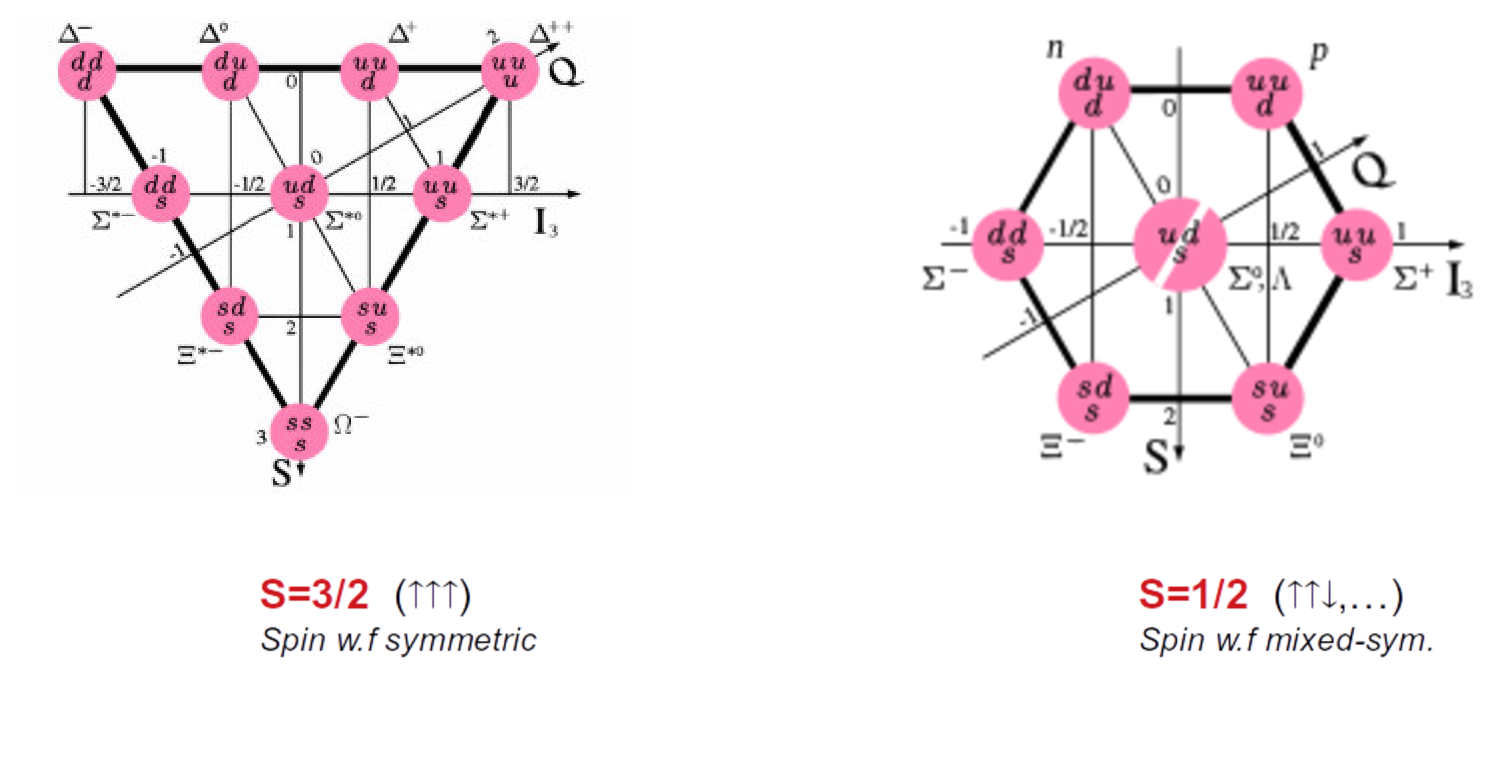
\includegraphics[width=0.9 \linewidth]{Chapter_introduction/eightfolds.eps}
  \caption{The eightfolds proposed by Gell-Mann and Ne'eman in 1961 to clasyfy baryonic states. At a publication moment they classyfy all known baryions except the $\Omega^-$. Its discovery in 1964 \cite{omega} was a great success of the quark model. }
  \label{fig:eigh}
\end{figure}

The quark modell is very succesful in a description of the baryonic ground states. However it gives no clue about excited states and quarks dynamics inside a particle. Because lattice QCD is still not able to reproduce even ground states masses the hyperons spectrum is calculated using effective theoris [ref]. Despite a huge theoretical end experimental effort a theoretical predictions and experimental data are still far away from agreement, especially in high mass range. The example of such is presented in fig. \ref{fig:spectrum}.

\begin{figure}[hb]
  \centering
  \includegraphics[width=0.99 \linewidth]{Chapter_introduction/spectrum.png}
  \caption{The comparison of experimental data (middle column) and theoretical predictions (left, and right column) of relativistically covariant constituent quark models for $\Lambda$ hyperons. The picture shows how limited is our experimental knowledge compare to theroetical predictions. The picture is taken from \cite{Ronniger2012}}
  \label{fig:spectrum}
\end{figure}
\section{Form factors}
Any kind of a scattering experiment performed to examinate physics inside baryions faces a fundamental problem of a rich internal structure of them. An complicated interactions inside the baryon can be treatet together and their inpact on a scattering could be take into consideration by one scalar function called a form factor F(q),
\begin{equation}
  \frac{d \sigma}{d \Omega}=\left( \frac{d \sigma}{d \Omega}\right)_{point-like} |F(\vec{q})|^2.
\end{equation}
As long as a target is static and spin-less the form factor is a the Fourier Transform of the charge decsity in target,
\begin{equation}
  F(\vec{q})=\int \rho(\vec{x}) e^{i \vec{q} \cdot \vec{x}}d^3x.
\end{equation}
Practically this relation occures whent a target is much heavier than a projectle, like in Rutheford experiment \cite{Rutheford}. In case of electron on proton scattering situation is more complicated because both particles has a spin and a proton gets recoil after scattering. A solution for this problem is called the Rosenbluth formula and looks as follows
\begin{equation}
  \frac{d \sigma}{d \Omega}\bigg|_{lab}=\left(\frac{\alpha^2}{4E^2 \mathrm{sin}^4 \frac{\theta}{2}}\right) \frac{E'}{E} \left[ \left(F_1(q^2)^2- \frac{\kappa^2 q^2}{4M^2} F_2(q^2)^2\right) \mathrm{cos}^2\frac{\theta}{2}-\frac{q^2}{2M^2} \left(F_1(q^2) + \kappa F_2(q^2)\right)^2 \mathrm{sin}^2 \frac{\theta}{2} \right],
\end{equation}
where $F_1(q^2)$ and $F_2(q^2)$ are two independent form factors, $\kappa$ anomalus magnetic moment, $q$ a four-momentum transfer. Factor
\begin{equation}
  \frac{E'}{E}=\frac{1}{1+\frac{2E}{M}\mathrm{sin}^2\frac{\theta}{2}}
\end{equation}
is conected with the proton recoil. Because functions $F_1$ and $F_2$ form an interference term it is convinient to express them as a linear combination of $G_e$ and $G_M$.
\begin{equation}
  G_e=F_1+\frac{\kappa q^2}{4M^2}F_2
\end{equation}
\begin{equation}
  G_M=F_1+\kappa F_2
\end{equation}

\section{Dalitz decays}
The idea of form-fastrs was introduced first time in context of scattering experiments. A Faynmann diagram for such phenomena is shown in fig. \ref{fig:FF_kinds} a). Due to kinematic constrains for the scattering a four-momentum $q^2$ is always negative - a projectile transfers part of its four-momentum into target. However an idea of the form factor can be extendet to annichilation experiments, where $q^2>0$ (fig.\ref{fig:FF_kinds} b)). Unfortunatelly, to produce a baryion-antybaryion pair energy equal at least their mases is reqired. It measns that $q^2$ can not be smaller than $4M_b^2$. This gap in $q^2$ can be explored in a range $0<q^2<4M_b^2$ by process called a Dalitz decay. 

\begin{figure}[hb]
  \centering
  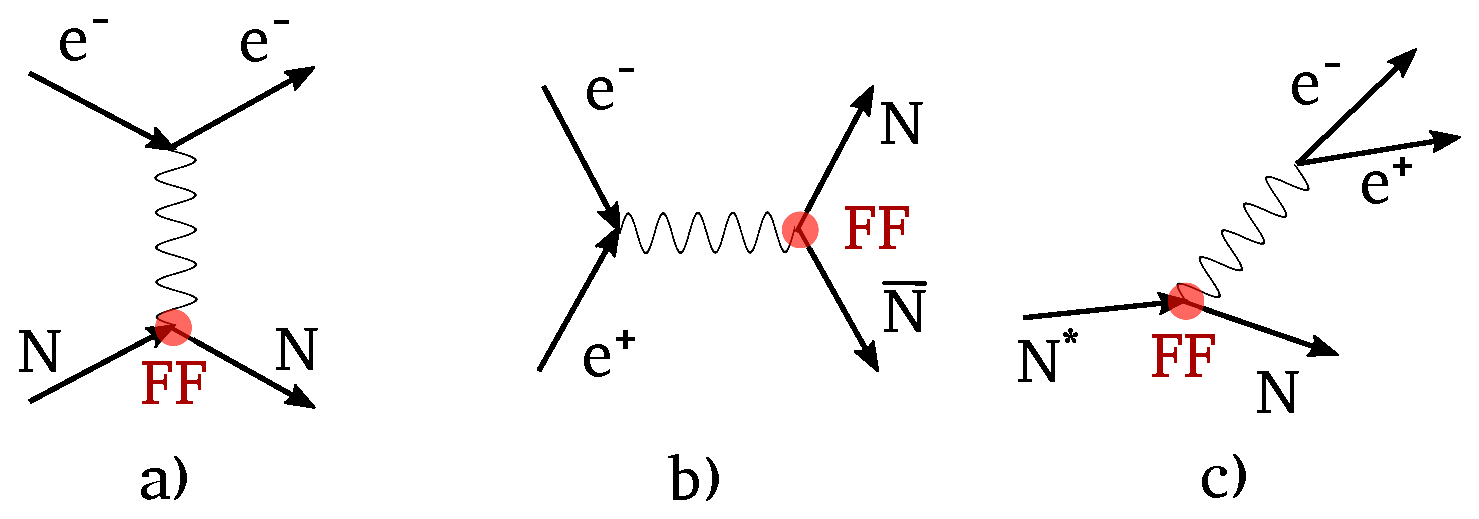
\includegraphics[width=0.9 \linewidth]{Chapter_introduction/faynmannDiagrams.eps}
  \caption{Three processes involving a nucleon electromagnetic form factors: a) an electron-nucleon scattering, b) an electron-positron anichilation, c) a nucleon Dalitz decay.}
  \label{fig:FF_kinds}
\end{figure}

The Dalitz decay of a nucleon ( is fig.\ref{fig:FF_kinds} c)) is a reaction 
\chapter{The HADES detector}
\label{chapter:detector}
The \textbf{H}igh \textbf{A}cceptance \textbf{D}i-\textbf{E}lectron \textbf{S}pectrometer (HADES) \cite{Agakishiev:2009am} is located at the GSI Helmholtzzentrum f{\"u}r Schwerionenforschung. The HADES detector was designed for various measurements with the especial emphasis on di-electron spectroscopy. Thanks to versatility of the SIS18 (German: \textbf{S}chwer\textbf{I}onen\textbf{S}ynchrotron) accelerator and a secondary pion beam facility, various kind of experiments can be conducted: starting from pion scattering on proton or nucleus targets, through proton-proton and proton-nucleus reactions, up to the heavy ion collisions. Up to now following experiments have been performed: C+C@2~GeV/u, p+p@2.2~GeV, Ca+KCl@2~GeV/u, C+C@2~GeV, Ar+KCl@1.765~GeV/u, p+p@1.25~GeV, p+p@3.5~GeV, d+p@1.25~GeV/u, p+Nb@3.5~GeV/u, Au+Au@1.23~GeV/u, $\pim$+$\mathrm{C_2H_4}$@1.7~GeV/u, Ag+Ag@1.58~GeV/u.

The detector provides almost full azimuntal angular coverage, whereas the acceptance in the polar angle used to rate from 18$^{\circ}$  to 80$^{\circ}$. A current upgrade extands the detector acceptance for forwards angles, for more detaisl see \ref{subsec:FwDet}. Two sets of toroidal \textbf{M}ulti-wire \textbf{D}rift \textbf{C}hambers (MDC) together with a superconducting toroid magnet allow for momentum measurements with $\frac{dp}{p} \approx 2-3\%$ and particle identification (PID) via energy loss measurement. The PID is further enhanced by high resolution \textbf{T}ime \textbf{O}f \textbf{F}light (TOF) detectors ($\sigma \approx 80$ ps) and a hadron-blind \textbf{R}ing \textbf{I}maging \textbf{CH}erenkov (RICH) detector. A combined information form the detectors allow for efficient p/$\pi$/K/e separation over broad momentum range. Even though it isn't a $4 \pi$ detector, thanks to its geometry it has acceptance around 40\% for pions produced in elementary collisions at energfys provided by SIS18 detector.
\begin{figure}
  \centering
  \includegraphics[width=0.7 \linewidth]{Chapter_detector/detector.eps}
  \caption{The HADES - \cs throug the detector. All essential sub-sytems used during pp and pNb experiment are visible in the picture. The picture from \cite{Agakishiev:2009am}.}
\end{figure}

\section{Tracking system}
The HADES tracking system bases on four sets of a drift chambers. Two before and two after a magnetic field. First set is called inner MDC, the second outer MDC. Each single drift chamber has a trapezoidal shape and consist of 13 layers of wires. They create 6 layers of a drift cells. A shape of the sells and the wires dencity was optimalized to get the best momentum resolutions.

Inbetween iner- and outer-MDC the \textbf{I}ron\textbf{L}ess \textbf{S}uperconducting Electron (ILSE) magen is located. It consist of six superconducting coils, which produce a toroidal magnetic field of 3.6 T inside the coils. The operational current can variy from 0 to 3500 A. 

The magnetic field produced by ILSE bends particles' tracks what allows for a momentum reconstruction. Tracks reconstruced in iner- and outer-MDCs have to be matched together. A deticated algorithm for this purpuse was developed by HADES collaboration. 

\section{META detectors}
A META detector during pp and pNb experiments consisted of two time of flight detectors: TOF and TOFino


\section{RICH detector}
The \textbf{R}ing \textbf{I}maging \textbf{CH}erenkov detector is the main tool for $\epem$ identyfication for the HADES. The detector active area surrounds target area and it is filled by a radiator gas ($\mathrm{C}_4 \mathrm{F}_{10}$). A refractive index gives a thrashold speed for a Cherenkov radiation production $\gamma_{thr} =18$. For projectile energys delivered by the SIS18 only particles able to exceed the threshold are electrons end positons. Passing across the radiator they produce a cone of a cherenkov light. Then, the light is reflected by a spherical mirror and detected by a pad plane located upstream a beam. An special algorithm called ''ring finder'' \cite{hades_RICH} reconstructs cherenkov light rings from a pattern of fired pads. A reconstructed ring position is mached with track from MDC to assign information about a leptonic character to proper track.  The detector is completelly ''hadronic blind'' what means that no hadron can give an signal in it. In 2019 the RICH was updated by a new readout system, described more detailed in next section. 
\begin{figure}
  \centering
  \includegraphics[width=0.6 \linewidth]{Chapter_detector/RICH.png}
  \caption{The \cs of the RICH detector.}
\end{figure}
\section{The HADES upgrades}

\subsection{The Forward Detector}
\label{subsec:FwDet}
In many studies especially devoted to hyperons' decays the forward angles play very important role. The hades detector for a quite long time did not have a possibility to register particles 
\subsection{RICH update}

\subsection{Electromagnetic calorimeter}

\label{chapter:HADES_upgrades}
\newcommand{\h}{$h(\vec{x})$}
\newcommand{\e}{\epsilon}
\chapter{Neural networks}\label{chapter:NN}



\section{The ROC curve and the optimal classifier}
One of the most common problem in machine learning is a binary classification, when a data set has to be divided into two subsets, fulfiling serian requirements. A simple example of such a problem is distinction between signal and bacground events in deta collected by experiment. We would like to have a function which takes as agruments set of physical observables (eg. particles' energy, momentum, coordinates of vertexes), represents by $\vec{x}$ and returns sigle number. More formally, a clasyfier can be call any function $h: \vec x \rightarrow \mathbb{R}$ designed in such a way, that high \h values correspond signal events and low \h values correspond background event. In most cases a classyfier output is squeezed by activation function to some finate range, for example from 0 to 1. A threshold value  \h =c, which is the value separating signal and backgrond events is called a working point, and has to be set by a user. The signal efficiency will be defined as $\e_S=\int d\vec x \rho_S(\vec x) \Theta(h(\vec x) -c)$ and respectively a background efficiency $\e_B=\int d\vec x \rho_B(\vec x) \Theta(h(\vec x) -c)$.

Problems: how to represent a clasyfier performence, how to compare different clasyfiers and how to choose proper working point have been discused since many years. During World War II engeeners faced a probelm of a radar detection efficiency. With an increasing radar sensitivity a chance to detect an enemy aircraft increses. However, the chanse that signal is a fake caused by birds or other circumstances also increases. To represent this relation a so-colled ROC (\textbf{R}eceiver \textbf{O}perating \textbf{C}haracteristic curve) curve was invited. One axis represents a true positive rate  or a detection efficiency, second axis shows a background reduction. Each point on the curve represents working-point for the clasyfier. Comparing two different classyfiers someone can not compare performance for one working point, but has to compare all. Graphic reprezentation of compared classyficators can be given by ROC curves.

\begin{figure}[hb]
  \centering
  %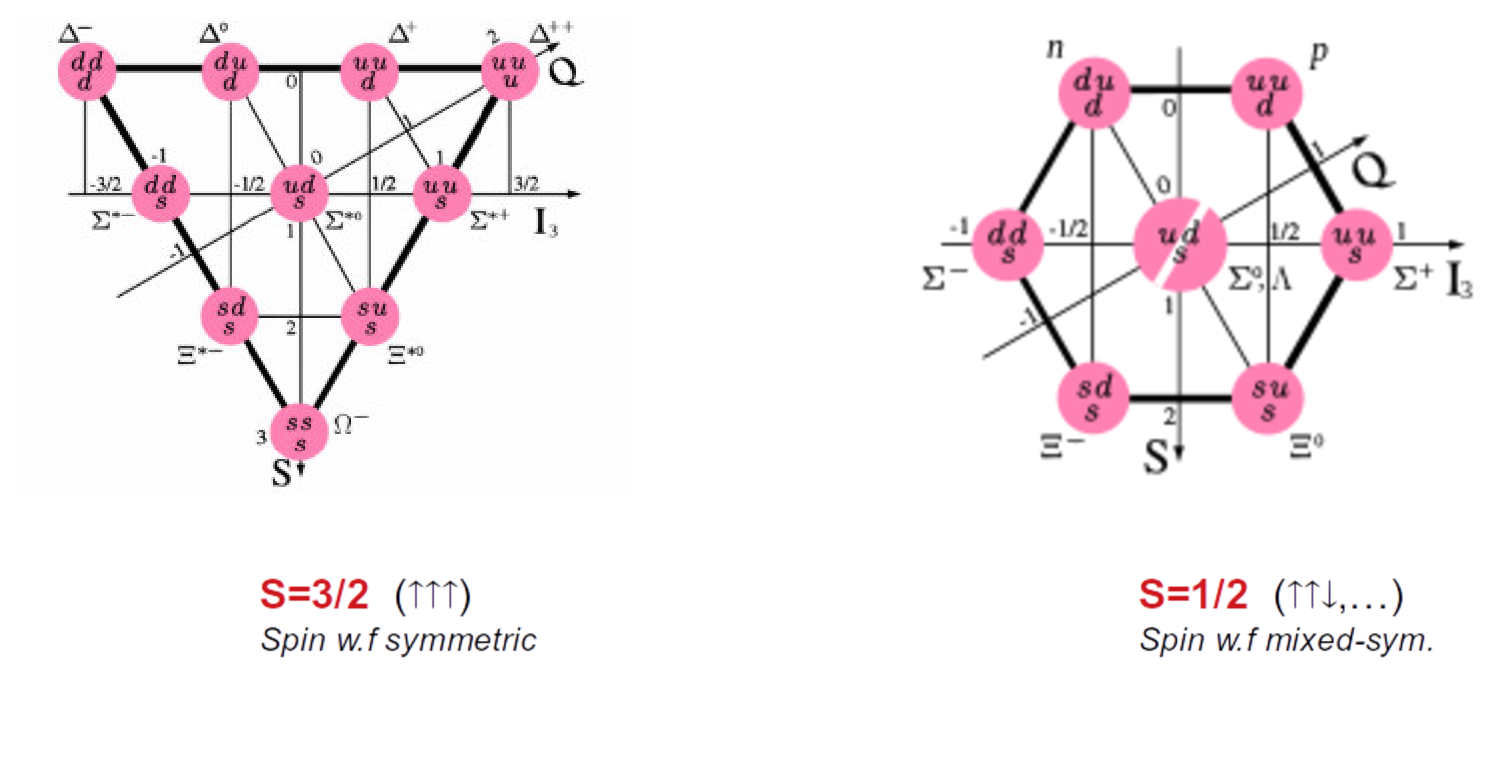
\includegraphics[width=0.9 \linewidth]{Chapter_introduction/eightfolds.eps}
  \caption{The ROC curve, it represents a clasyfier performence. In case of the ideal clasyfier area under the curve is equal 1, what means that for each working point all background events are rejected and non of singal is lost. }
  \label{fig:ROC}
\end{figure}

The optimal clasyfier is deffined as
\begin{equation}
  \forall c \forall \e_S
\end{equation}

In graphical approach the ptimal classyfier should give the biggest area under the ROC curve from all possible classyfiers. In case of complitly separable sets of data the area should be equal 1.
\section{The data-driven approach}
The original paper by Metodiev, Nachman and Thaler \cite{Metodiev_2017} the othors show the idea of a data-driven analysis in details. In this chapter I want to introduce main concepts, necessery to understand how the proposed metode helps in week decays recosntruction.

In a classical approach to supervized machine learning, a model learns its properties usign sets of labeled data. Of courese providing good training sets is always a problem. To do this, someone can use either experimental data, labeled by a user, or simulation. In first case a user uses his external knowledge about the data to describe it. In second case the user fully rely on simulation. First case is quite often impossible to perform, but even when a user is able to label data a labeling could be systematiclly biased by a lack of knowlage or missunderstand of detector. In second case they are two main threats: either a simulation does not describe data well, or creates some artificial structures in data, which can lead into sistematic errors in network performence. 

The data-data driven analysis avoids inconveniencees of two mentioned methodes. It requires neither labeling nor simulation and it bases only on statistical properties of a collected deta set. According to Neyman-Pearson lemma \cite{Neyman-Pearson} the optimal clasyfier for two sets, A and B is a function given by a dencity ratio
\begin{equation}
  \label{eq:N-P}
  h_{opt}^{A/B}(\vec x)=\frac{\rho_A}{\rho_B}
\end{equation}
or any monotonous function of $\frac{\rho_A}{\rho_B}$. Assuming that both sets A and B contains signal (s) and bacground (b) events and a statistical distribution of s and b is the same in A and B, we can write \eqref{eq:N-P} in the following way
\begin{equation}
  h^{A/B}_{opt}=\frac{f_1 \rho_s + (1-f_1) \rho_b}{f_2 \rho_s + (1-f_2) \rho_b}=\frac{f_1 \rho_s/\rho_b+1-f_1}{f_2 \rho_s/\rho_b+1-f_2}=\frac{f_1 h_{opt}^{s/b}+1-f_1}{f_2 h_{opt}^{s/b} +1-f_2}.
\end{equation}
It can be proven that $\partial_{h_{opt}^{s/b}}h_{opt}^{A/B} >0$, what means that optimal clasyfier for both cases is the same, so the clasyfier trained to distinguish A and B should also gives some separation power between signal and background. The situation is represented graphically in fig. \cite{fig:DD}.  It is important to underline that the reasoning gives no clue about the working points for both cases. 

\begin{figure}[h]
  \centering
  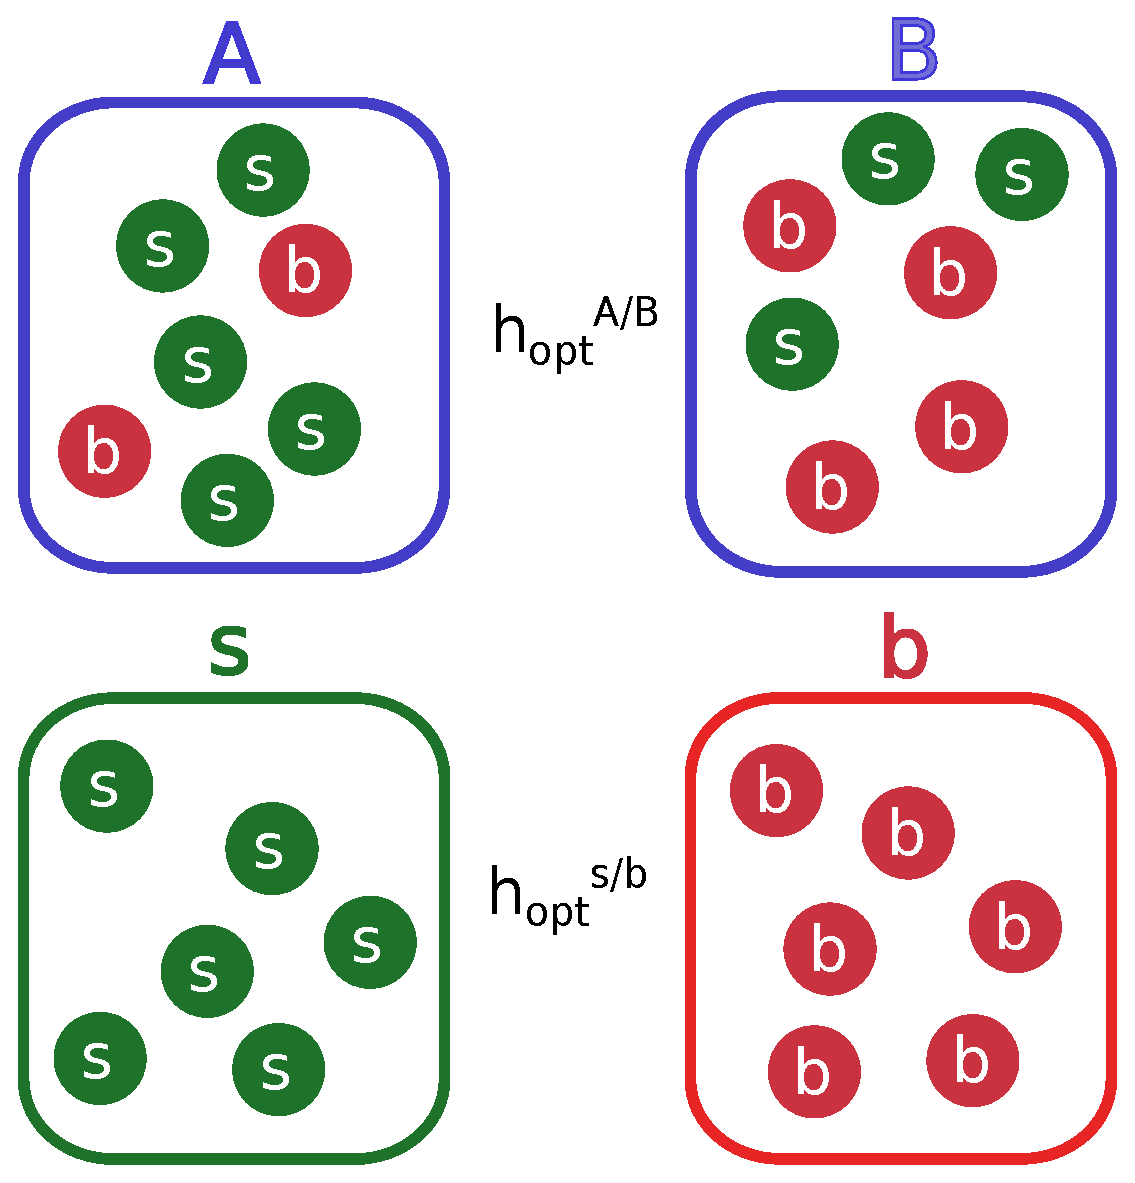
\includegraphics[width=0.5 \textwidth]{Chapter_NN/setAB.eps}
\caption{A data-driven approach visualisation. According to \cite{Metodiev_2017} the opitimal clasyfier for sets A and B is equivalent to optimal clasyfier for sets s and b.}
\label{fig:DD}
\end{figure}



\section{Application for analysis}
In case of $\Ls$ reconstruction the data driven approach was used to replace set of geometrical cuts and enchace a $\Lz$ signal~to~background ratio. So for the neural network all events with $\Lz$ were treated as a signal and without like a background. For all events an invariant mas of $\p \pim$ pair was ploted (fig. \ref{fig:L1116_DD}). Using this spectrun the dataset was divided in two subsets: for $M^{inv}_{\p\pim} \in (1015,1125)$ and $M^{inv}_{\p\pim} \notin (1015,1125)$. In the first of them a ratio between $\Lz$ and background is clearly different than in the second, what fulfil the requariments for the data-driven aproach. Hence, a numerous networka architecture were tested to check which deals the best with $\Lz$ reconstruction.

\begin{figure}[ht]
  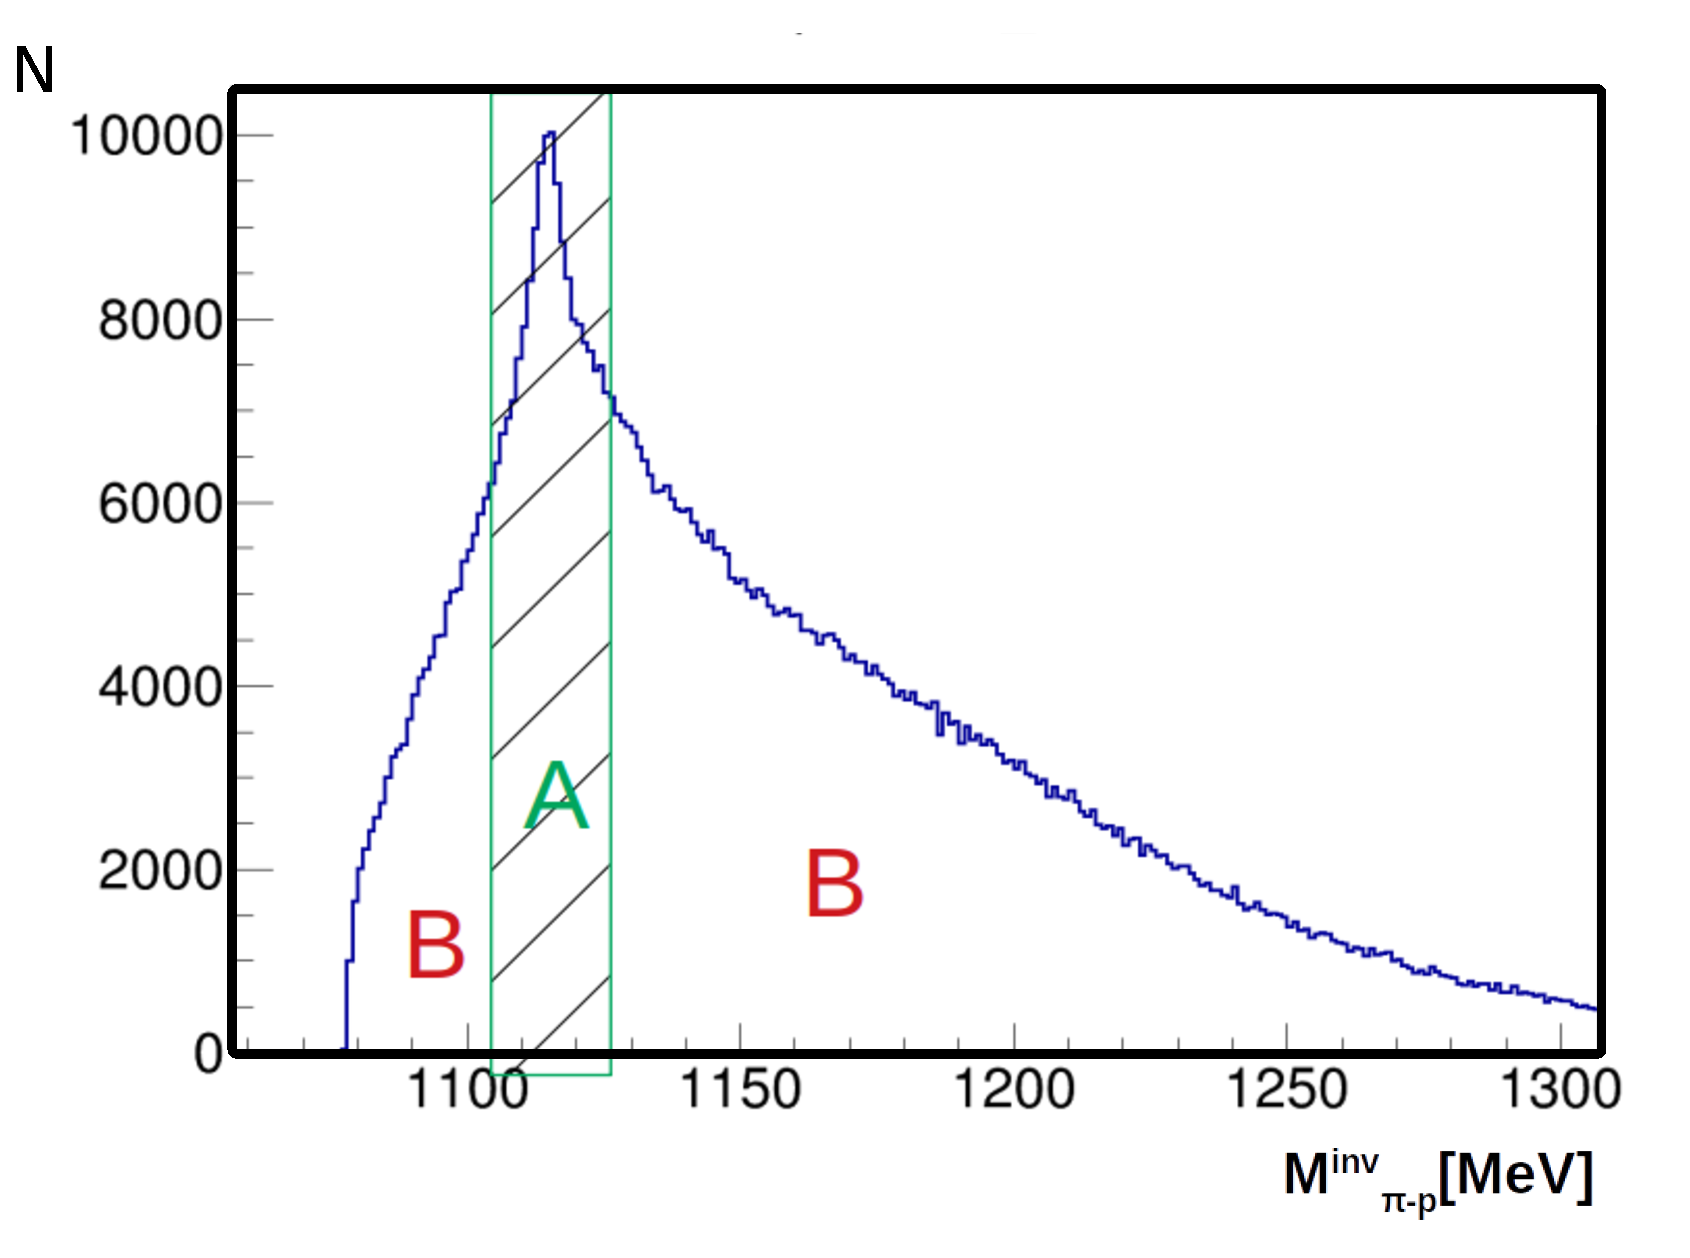
\includegraphics[width=0.8 \textwidth]{Chapter_NN/L1116.eps}
  \caption{A $\p \pim$ invariant mass specrum. Whole data set was divided into two subsets, A and B, each of them is characterized by different signal~to~background ratio. All tested models were trained to distinguish between sets A and B and later use to seperate events containing $\Lz$.}
  \label{fig:L1116_DD}
\end{figure}

A learning and testing proces was done within scope of TMVA framework \cite{TMVA}. Using TMVA a user has to provide list of input variables and a network architecture, than the framework automaticly preperes learning and testing sets and performs whole learning process together with testing the final classyfier. As an input variables the set of geometrical properties was used.
\begin{itemize}
\item Distance between $\p \pim$
\item $\Lz$ vertex cooridanes, reconstructed as a point of the closest aproach of $\p$ and $\pim$ tracks
\item $\Ls$ vertex coordinates, rseconstructed as a point of the closest approach of $\pip$ and $\pim$ tracks
\item $\Ls$ vertex coordinates, reconstructed by tracking algorithm as a primary vertex
\item Opaning angle between reconstructed $\Lz$ vector and a line conecting primary and secondary verteces
\end{itemize}
Using any combination of input variables it is impossile to reconstruct $\p \pim$ invariant mass. It is important feature wich allows to use mesioned invariant mass spectrum as a cross-check for all procedure, and a network will not collapse into trivial solution.

During treaning the network is optymalized to seperate sets A and B. Its performence for $\Lz$ reconstruction has to be investigated in a different way. After the traning the network was used to evaluate each event collected during the experiment. It means, that network output - a number in range from 0 to 1 - is assigned to each reconstructed event. Fitting a $\Lz$ peak (see \ref{fig:NN_wynik} a)) it was possible to check how signal efficiency and signal~to~background ratio changes with cut on the network output.

\begin{figure}[ht]
  \centering
  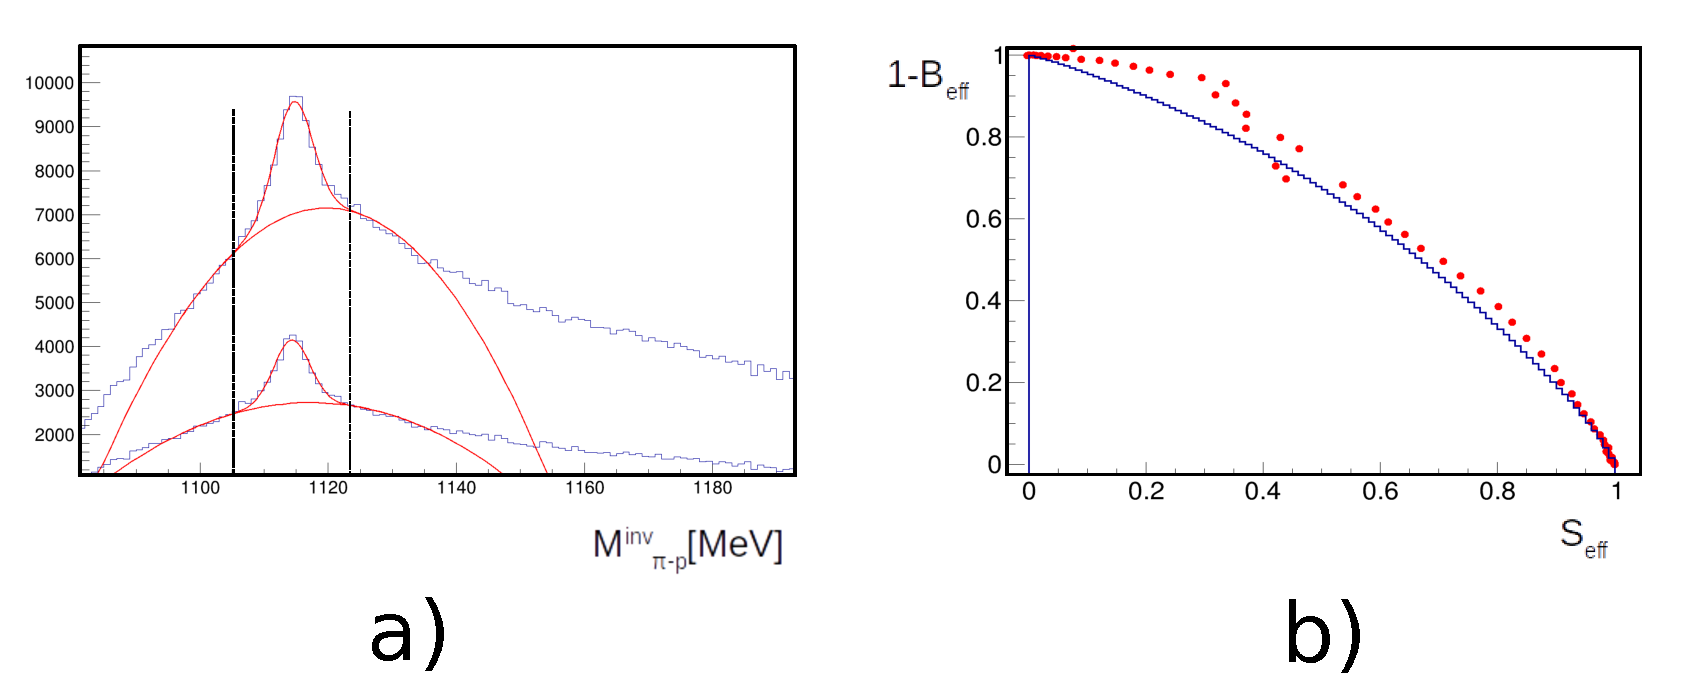
\includegraphics[width=0.9 \textwidth]{Chapter_NN/NN_wyniki.eps}
  \caption{Results of a neural network training. a)Example of two spactra after a cut on the network output. For each of the the signal (gausian function) and background (4-th order polynomial) were fitted. Such fits allows to calculate a signal efficiency $\frac{S}{S_0}$ and a background rejection $1-\frac{B}{B_0}$, where $S_0$ and $B_0$ are yelds of signal and background without any cut on a neural network output. }
  \label{fig:NN_wynik}
\end{figure}

%%% Local Variables:
%%% TeX-master: "../main"
%%% End: 
\chapter{Deta analysis}
\label{chapter:analysis}
The HADES experiment has performed a proton-proton experiment with beam kinetic energy 3.5 GeV in September 2018. Data collected during this experperiment allowed to conduct a series of analysis devoted to hypererons [ref]. In this thesis the next step in hyperon studies is presented. The four particles $\p \pim \pip \pim$ final state was analyzed. Is allows to reconstruct the inclusive signal of $\Ls$ and $\Lz \Kz$ signal. The obtained results were compared with previous, exclusive measurements and used to constrain simulation of a new esperiment devoted to hyperon studies \ref{chapter:simulations}.

All methodes developed for pp@3.5 GeV experiment were used for deta from pNb@3.5GeV experiment. A simirar analysis ..

\section{Paricles identyfication}
The HADES detector allows for two complementary methodes of particles analysis. A first of them bases on particles time of flight measured in the TOF detectors and particle's momentum measured in the MDC. A second methode bases on MDC exclusively and uses combide information about particles' momentum and energy losses. The first one is favoured due to better precision, however a limited geometrical of the TOF detectors reduces detection efficirncy by a factor 0.8 for each particle. In case of four particles final state, discussed in this thesis, a total loss caused by the TOF detectors  can reach 60\% of all detected particles. For that reason the $\frac{de}{dx}$ vs. momentum identyfication metode was used. Cuts were opimized in Munich group involved in HADES experiment and described in.[ref].
\section{Absolute normalization}
\label{sec:normalization}
An integrated luminosity for the pp experiment was calculated by a pp elastic scattering. It was
\begin{equation}
  L^{int}=3.13 \cdot 10^8 mb^{-1}.
\end{equation}
Thanks to a full scale simulation performed in HYDRA framework it is posible to get a total detection efiiciency for given reaction. Together with a luminocity its provide an ecpected count rate for each channel
\begin{equation}
  N^{\mathrm{expected}}_{pp\rightarrow X}=\frac{N_{\mathrm{detected}}}{N_{\mathrm{Simulated \; in \;} 4 \pi} \cdot 3} \cdot \sigma_{pp\rightarrow X} \cdot L.
\end{equation}
The factor 3 in denominator is connected with a trigger down-scaling. For a hadronic channels each 3th triggered event was seved on tapes. A list of the \css used in following analysis are in \ref{tab:channels}. 
\begin{table}
    \centering
  \caption{List of the channels considered in following chapter. Numbers from 3 up to 10 indicates reactions containing $\p \pim \pip \pim$ in a final state. They are treated as a possible background channels. All values taken from \cite{hades_inclL_35}.}
  \label{tab:channels}
  \begin{tabular}{rll}
    \hline
    no. &Channel & $\sigma$ [$\mu \barn$]\\
    \hline
    \hline
    \multicolumn{3}{c}{3-body reactions} \\
    \hline
    1 & $\Lz \p \Kp$&$35.26 \pm 0.43 ^{+3.55}_{-2.83}$\\
    2 & $\Sz \p \Kp$&$16.5 \pm 20\%$\\
    3 & $\Lz \Dpp \Kz$&$29.45\pm 0.08 ^{+1.67}_{-1.46}\pm 2.06$\\
    4 & $\Sz \Dpp \Kz$&$9.26 \pm 0.05 ^{+1.41} _{0.31}\pm 0.65$\\
    5 & $\Sigma(1385)^+ \p \Kz$&$14.05 \pm 0.05 ^{+1.79}_{-2.14}\pm 1.00$\\
    6 & $\Dpp \Lss \Kz$&$5.0\pm 20\%$\\
    7 &$\Dpp \Ss \Kz$& $3.5 \pm 20\%$\\
    8 &$\Dp \Sigma(1358)^+ \Kz$&$2.3 \pm 20\%$\\
    \hline
    \multicolumn{3}{c}{4-body reactions} \\
    \hline
    9 &$\Lambda \p \pip \Kz $& $2.57 \pm 0.02 ^{+0.21}_{-1.98}\pm 0.18$\\
    10&$\Sz \p \pip \Kz$& $1.35 \pm 0.02 ^{+0.10}_{-1.35}\pm 0.09$\\
    \hline
  \end{tabular}
  
\end{table}

\section{Event selection}
Among all registered events only these with at least four charged particles (two positive and two negative) has been registered in the HADES. In case of situation when detector registered more particles the combination with the lowest $\chi^2$ was taken. ...
\section{Reaction kinematics}
\label{section:kinematics}
A next step after an event selection  was a look into a missing mass spectrum of all analized events. Becouse the easiest production mechanism for a pp reaction is as follows
\begin{equation}
  \p\p \rightarrow \p \Kp \Lz,
\end{equation}
hence, for a $\Lz$ decaying int $\Ls \pip \pim$ a final states is
\begin{equation}
  \p\p\rightarrow \p \Kp \p \pim \pip \pim.
\end{equation}
The smallest missing mass for the signal channel is a sum of $\p$ and $\Kp$ mass. At the same time, for a main background source: a multipion production in a target, the smallest missing mass is equal a sum of $\p$ and $\pip$ mass. The missing mass spectrum is presented in fig. \ref{fig:missMass}.
\begin{figure}[hb]
  \centering
  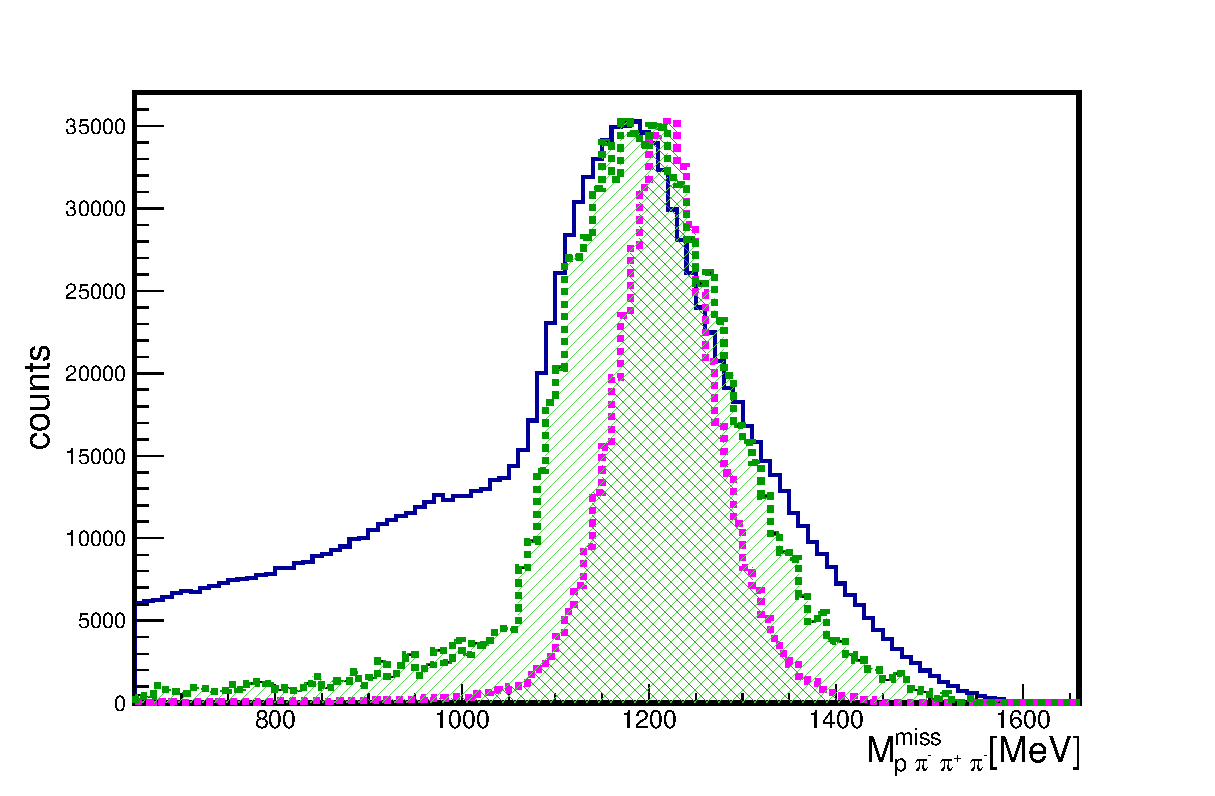
\includegraphics[width=0.9 \linewidth]{Chapter_analysis/missMass.eps}
  \caption{The missing mass of $\p \pim \pip \pim$ system. The resonance behavour around 1200 MeV is cleary visible. The read line represents sum of signal (a Voigt function) and a background (5-th order polynomial) fit. Fited Voigt function gives following parameters: $\bar{M}=1186$ MeV, $\sigma=61$ MeV, $\Gamma=$20 MeV.}
  \label{fig:missMass}
\end{figure}
Becouse in HADES energy regime almost all pions are produced via resonances tit was expected that together with $\Dpp$ visible in missing mas a simiral signal should bi visible in $\p \pip$ invariant mass spectrum. Indeed, as it is shownn in fig. \ref{fig:dpp2D} most of the background comes from coreleted source. The figure shows also that a cut on missing mass > xxx rmuves a significant part of a background events.
\begin{figure}[hb]
  \centering
  %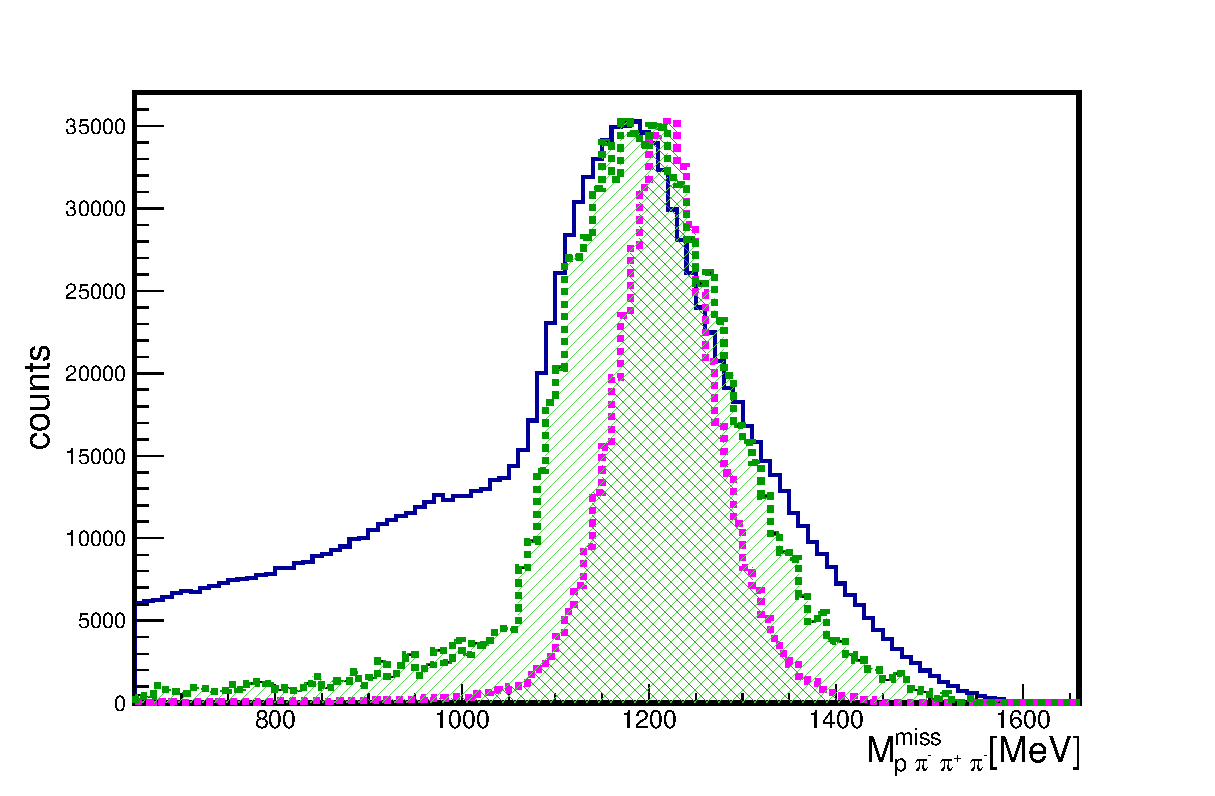
\includegraphics[width=0.9 \linewidth]{Chapter_analysis/missMass.eps}
  \caption{The missing mass of $\p \pim \pip \pim$ system vs. invariant mass of a $\p\pim$ system. It is creary visible that most of the bacground comes from corelated source of two $\Dpp$ production. Such situation helps to easy discriminate most of the background.}
  \label{fig:dpp2D}
\end{figure}

\section{The $\Lz$ Reconstruction}
The next step of the analysis after a missing mass cut was a $\Lz$ reconstructiion. In previous HADES experiments the reconstruction bases on a set of geometrical cuts. Their role was to increase signal-to-background ratio utlizing a $Lz$ decay gemetry. Because the $\Lz$ decasys via week interactions its livetime is relatively long :$c\tau = 7.89 cm$ \cite{PDG}. That may be used to discriminate an out of target vertex from a background originates from a target.

As it was shown in \ref{section:kinematics} an avaliable phase-space for $\Ls$ production for a $E_k=3.5$ GeV is very limited. An inlusive analysis performed in \cite{hades_L1520} has measured N events of $Ls$ after all cuts. To impruve statistics, and also axminate new reconstruction methodes in following analysis a neural network was used to replace the geometrical cuts. Details about used methode are explaned in chapter \ref{chapter:NN}.

The opitimalized neural network enhanced a signal to bacgkround ratio from ??? without any topological cuts to ???. A $\Lz$ signal obtained in this way was used for a next steps of analysis: the $\Ls$ analysis (chapter \ref{section:Ls}) and asocieted $\Lz \Kz$ production (chapter \ref{section:LzKz});
\section{The $\Ls$ Reconstruction}
\label{section:Ls}

\subsection{Side-band analysis}
\section{The $\Lz \Kz $reconstruction}
\label{section:LzKz}
Because of the conservation low a $\Lz$ has to be produced with some anti-strange particle. The lightest option is a $\Kz$ meson, which decays in 69.2\% into $pip pim$ pair \cite{PDG}. For that reason a $\Lz \Kz$ signal is expected to be a significant part of the $\Lz \pip \pim$ final state.

After the $\Lz$ reconstruction two spectra were drown: a) a $\pip \pim$ invariant mass spectrum for events $1006<M^{inv}_{\p \pim}<1026$ and b) a $p pim$ invariant mass for $480 MeV<M^{inv}_{\pip \pim}<500 MeV$. The same analysis chain was used to analyzed all channels from \ref{tab:channels} which contains $\Lz$ and $\Kz$. 

Using a procedure described in \ref{sec:normalization} the simulation was compared with experimental data (see \ref{fig:K0L0}). The simulation describes well a yeld of $\Kz$ and $\Lz$ produced in experiment, aldough it does not describe the background shape. ?? 

\begin{figure}[hb]
  \centering
  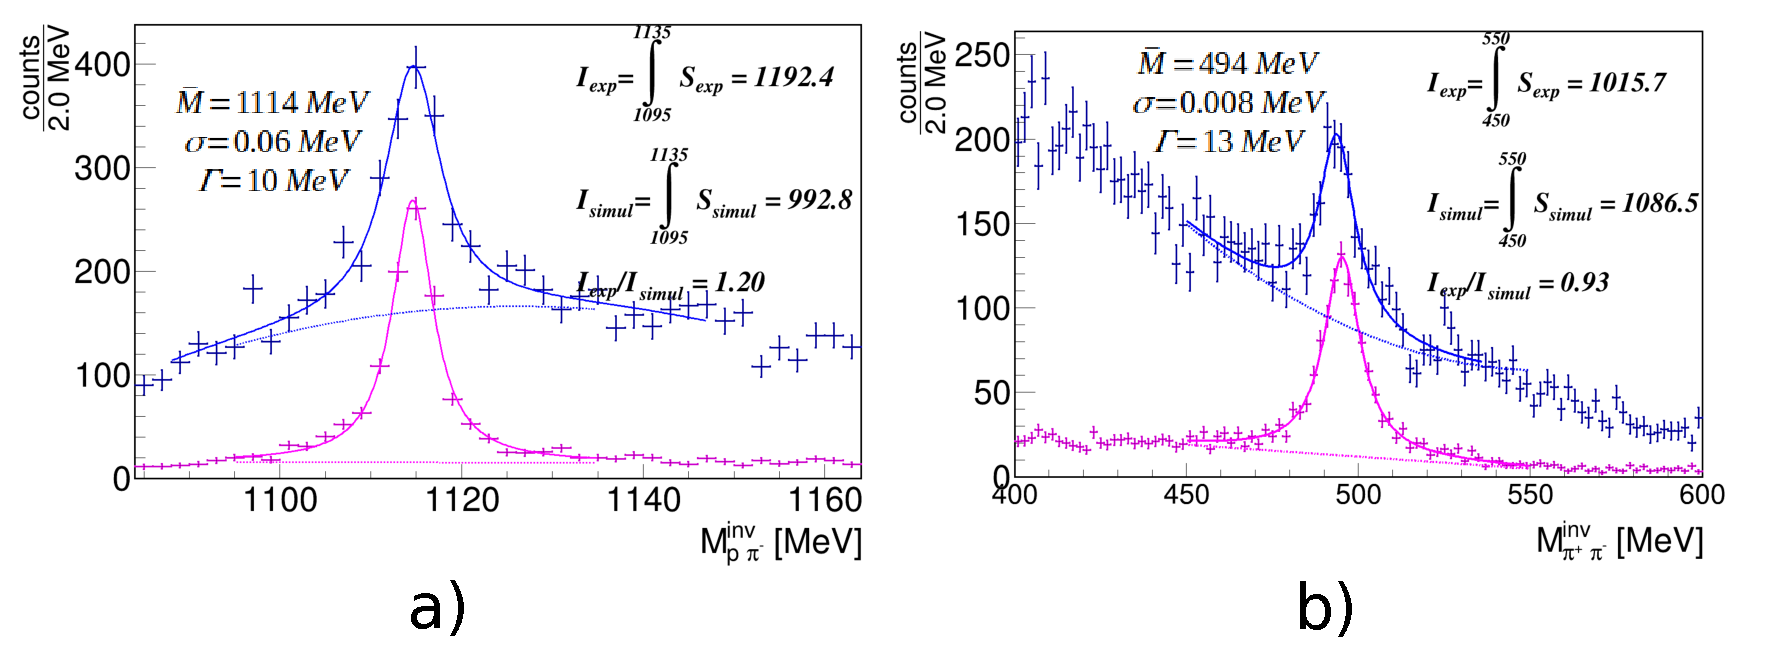
\includegraphics[width=0.9 \linewidth]{Chapter_analysis/K0L0.eps}
  \caption{The results for $\Lz \Kz$ asocieted production. Blue point reprezents experimental data, magenta a sum simulated channels. For both: the simulation and the experimental data a Voigt function was fited. Than a total signal yeld between simulation and experiment was calculated.}
  \label{fig:K0L0}
\end{figure}


\section{results from p Nb experiment}
\chapter{PNb data analysis}
\label{chapter:analysis_pNb}
As a result an inclusive \cs for $\Ls$ together with the reference state $\Lz \Kz$ were measured for prono-nucleus scattering. Compare to previous HADES studies \cite{hades_Sz_pNb,hades_Lp_femtoscopy_pNb,hades_arnold_pNb,hades_Ksi_pNb} it allows to extend knowladge about hyperons in pNb reactions.

\section{Identyfication and data selection}

\section{The $\Lz$ Reconstruction}


\section{The $\Lz \Kz $reconstruction}



\section{The $\Ls$ Reconstruction}



\subsection{Event mixing}


\subsection{Cross-section and extraction differential analysis}

\subsection{Analysis of a $\pip \pim$ spectrum}

\section{Comparison with results from pp data}
\chapter{Simulations of a new experiment}
\label{chapter:simulations}
The HADES collaboration is one of the leading forces of a FAIR Phase-0 project. Within the scope of the FAIR project a pp@4.5GeV experiment is going to be preformed. It gives a great opportunity to increase a knowledge about hyperons, with special emphasis on hyperons' Dalitz decays (see Chapter \ref{chapter:introduction}). One of the goals of my work was to carry out a simulation of such an experiment. The performed simulation was used as an input for proposal ubmited by HADES experiment for [nazwa komisji]. As the result the HADES was granted 4 week proton beem devoted for hyperons studies.
\section{An estimation of cross-sections}
In energy range of $1 \mathrm{GeV}<\Sqs<6 \mathrm{GeV}$ an exclusive \cs for $\Lz$ and $\Sz$ production were measured for many different energies \cite{hades_inclL_35,COSY-TOF_SigmaLambda,L-B}. Also an exclusive \cs for $\Lss$ production  was measured for two different energies \cite{hades_L1405,COSY-TOF_L1405}, and for $\Ls$, was measured once \cite{hades_inclL_35}. In contrast to the exclusive production \cs, inclusive \css for hyperons' production in pp collisions are poorly known. The first step to perform a reliable simulation was to estimate possible \css based on an available knowledge.

\subsection{$\Lz$ inclusive \cs}
The first step for all estimations is a parametrization of a $\Lz$ inclusive production. In a given energy range there are four measured values. More over, some additional assumptions can be made i) the production \cs is equal 0 for threshold energy, ii) for energy below one pion mass (140~MeV) the inclusive and the exclusive \css are the same. Hence, for the parametrization could be used an already measured inclusive \cs for $\p\p \rightarrow \p \Kp \Lz$ for $\Sqs$ below ??. To the all available data points meeting my requirements I fitted a 3th order polynomial
\begin{equation}
  \label{eq:L1116param}
  \sigma_{\p\p \rightarrow \Lz X}(\Sqs)=48 \cdot (\Sqs -2.55)+292.6 \cdot (\Sqs-2.55)^2-45.4 \cdot (\Sqs-2.55)^3.
\end{equation}
Fit result, together with residual plot is show in \ref{fig:inclusive_cs} by a blue dotted line. This parametrization forms the basis off all inclusive \css estimated in my work.

\subsection{$\Sz$ inclusive \cs}
According to PDG \cite{PDG} almost all $\Sz$s decay into $\Lz$. I means that the inclusive $\Lz$ signal contains a fraction deriving from $\Sz$ decays. However knowing a relation between $\Lz$ and $\Sz$ it is possible to disentangle both contributions.
\begin{figure}[hb]
  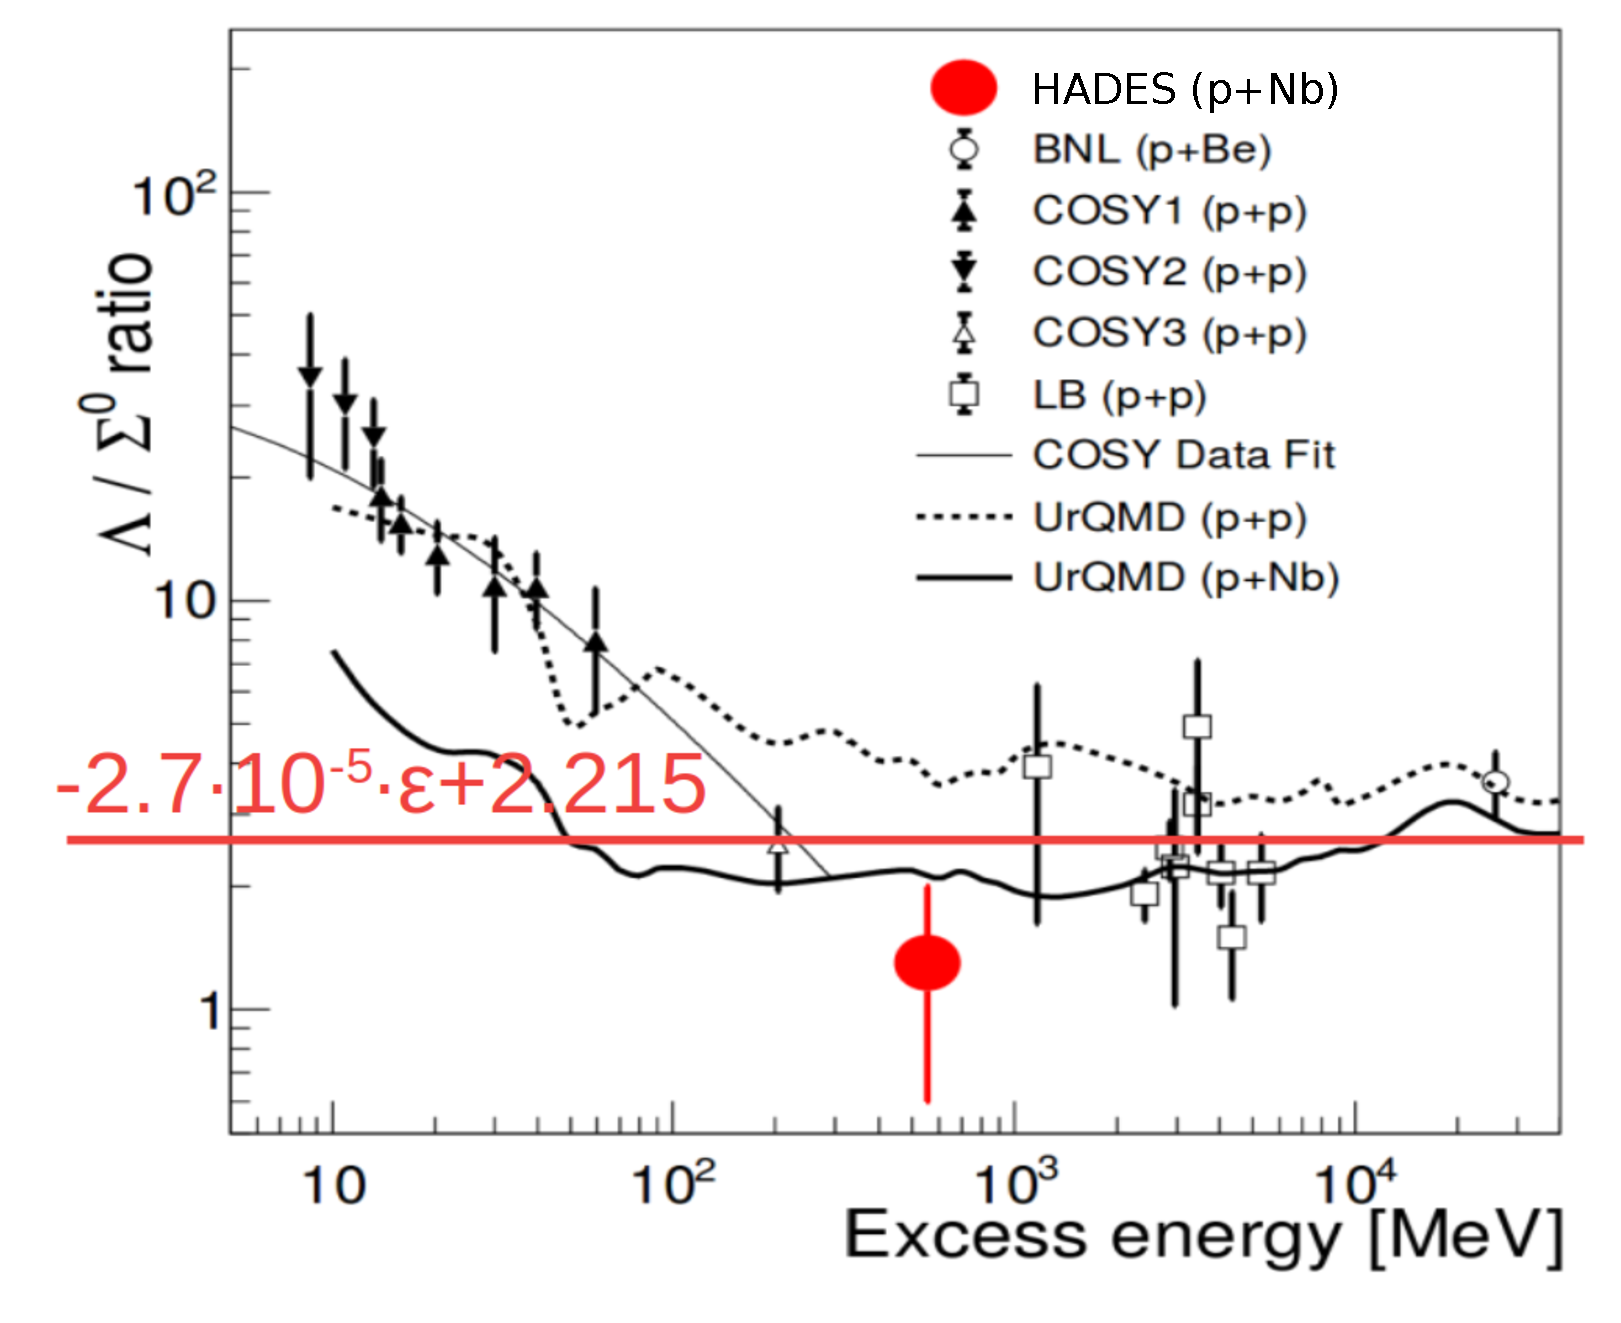
\includegraphics[width=0.6 \linewidth]{Chapter_simulation/LtoS.eps}
  \caption{A measeured ratio between $\Lz$ and $\Sz$ exclusive \cs. I low $\eps$ range the COSY-TOF parametrization was used, for $\eps > ???$ the data is described by liner function. The picture taken from \cite{hades_Sz_pNb}.}
  \label{fig:LtoS}
\end{figure}

A $\Sz/\Lz$ ratio was measured by COSY-TOF and others \cite{COSY-TOF_SigmaLambda}. Additionally the COSY-TOF collaboration proposed a parametrization of the ratio for access energy $\eps <200~\mathrm{MeV}$. Above this energy ($\eps >200~\mathrm{MeV}$) a linear parametrization 
\begin{equation}
  \frac{\Lz}{\Sz}(\eps)=2.215 - 2.7 \cdot 10^{-5} \eps
\end{equation}
describes data quite well ($\chi^2=0.89$). In fact for $\eps>200MeV$ the ratio is almost constant and does not depend on energy. For further calculations the COSY-TOF and the linear parametrizations were glued at ???.

Knowing the $\Lz/\Sz$ ration it is possible to disentangle a $\Lz$ and $\Sz$ production. Using determined ratio and the $\Lz$ production (let's call it~$P_1$) and  parametrization given by eq. \ref{eq:L1116param} (called~$P_2$), a following ste of equations is created 
\begin{equation}
  \label{eq:set_1}
  P_1(\eps)=\frac{L(\eps)}{\S(\eps)}=\frac{L(\Sqs - \Lz_{thr})}{\S(\Sqs - \Sz_{thr})}=P_1(\Sqs),
\end{equation}
\begin{equation}
  \label{eq:set_2}
  P_2(\Sqs)=\L(\Sqs)+\S(\Sqs),
\end{equation}
Where $\Sigma$ represents the inclusive $\Sz$ production \cs and  $\L$ the $\Lz$ \cs accordingly. Solving the first equation and shifting an argument by $\Sz_{thr}$ it is possible to obtain an equation,
\begin{equation}
  \label{eq:set_3}
  \S(\Sqs) \cdot P_1(\Sqs + \Sz_{thr})=\L(\Sqs - \Lz_{thr} +\Sz_{thr}).
\end{equation}
Now, using eq. \ref{eq:set_3} and \ref{eq:set_2} I got a recurrence relation
\begin{equation}
  \L(\Sqs - \Lz_{thr} +\Sz_{thr})=P_1(\Sqs +\Sz_{thr}) \left( P_2(\Sqs)-\L(\Sqs) \right).
\end{equation}
Assuming that $\L(\Lz_{thr})=0$ and $\S(\Sz_{thr})=0$, the above equation can be solved with any given precision. For the purpose of \css estimation a single step was set $\Delta M = \frac{\Sz_{thr}-\Lz_{thr}}{10}$, obtained decomposition is shown in \ref{fig:inclusive_cs} by dashed lines. A characteristic ``kick'' on the green line corresponds to energy when two parametrization of $\frac{\Lz}{\Sz}$ ratio are glued (see fig ??). 

\begin{figure}[hb]
  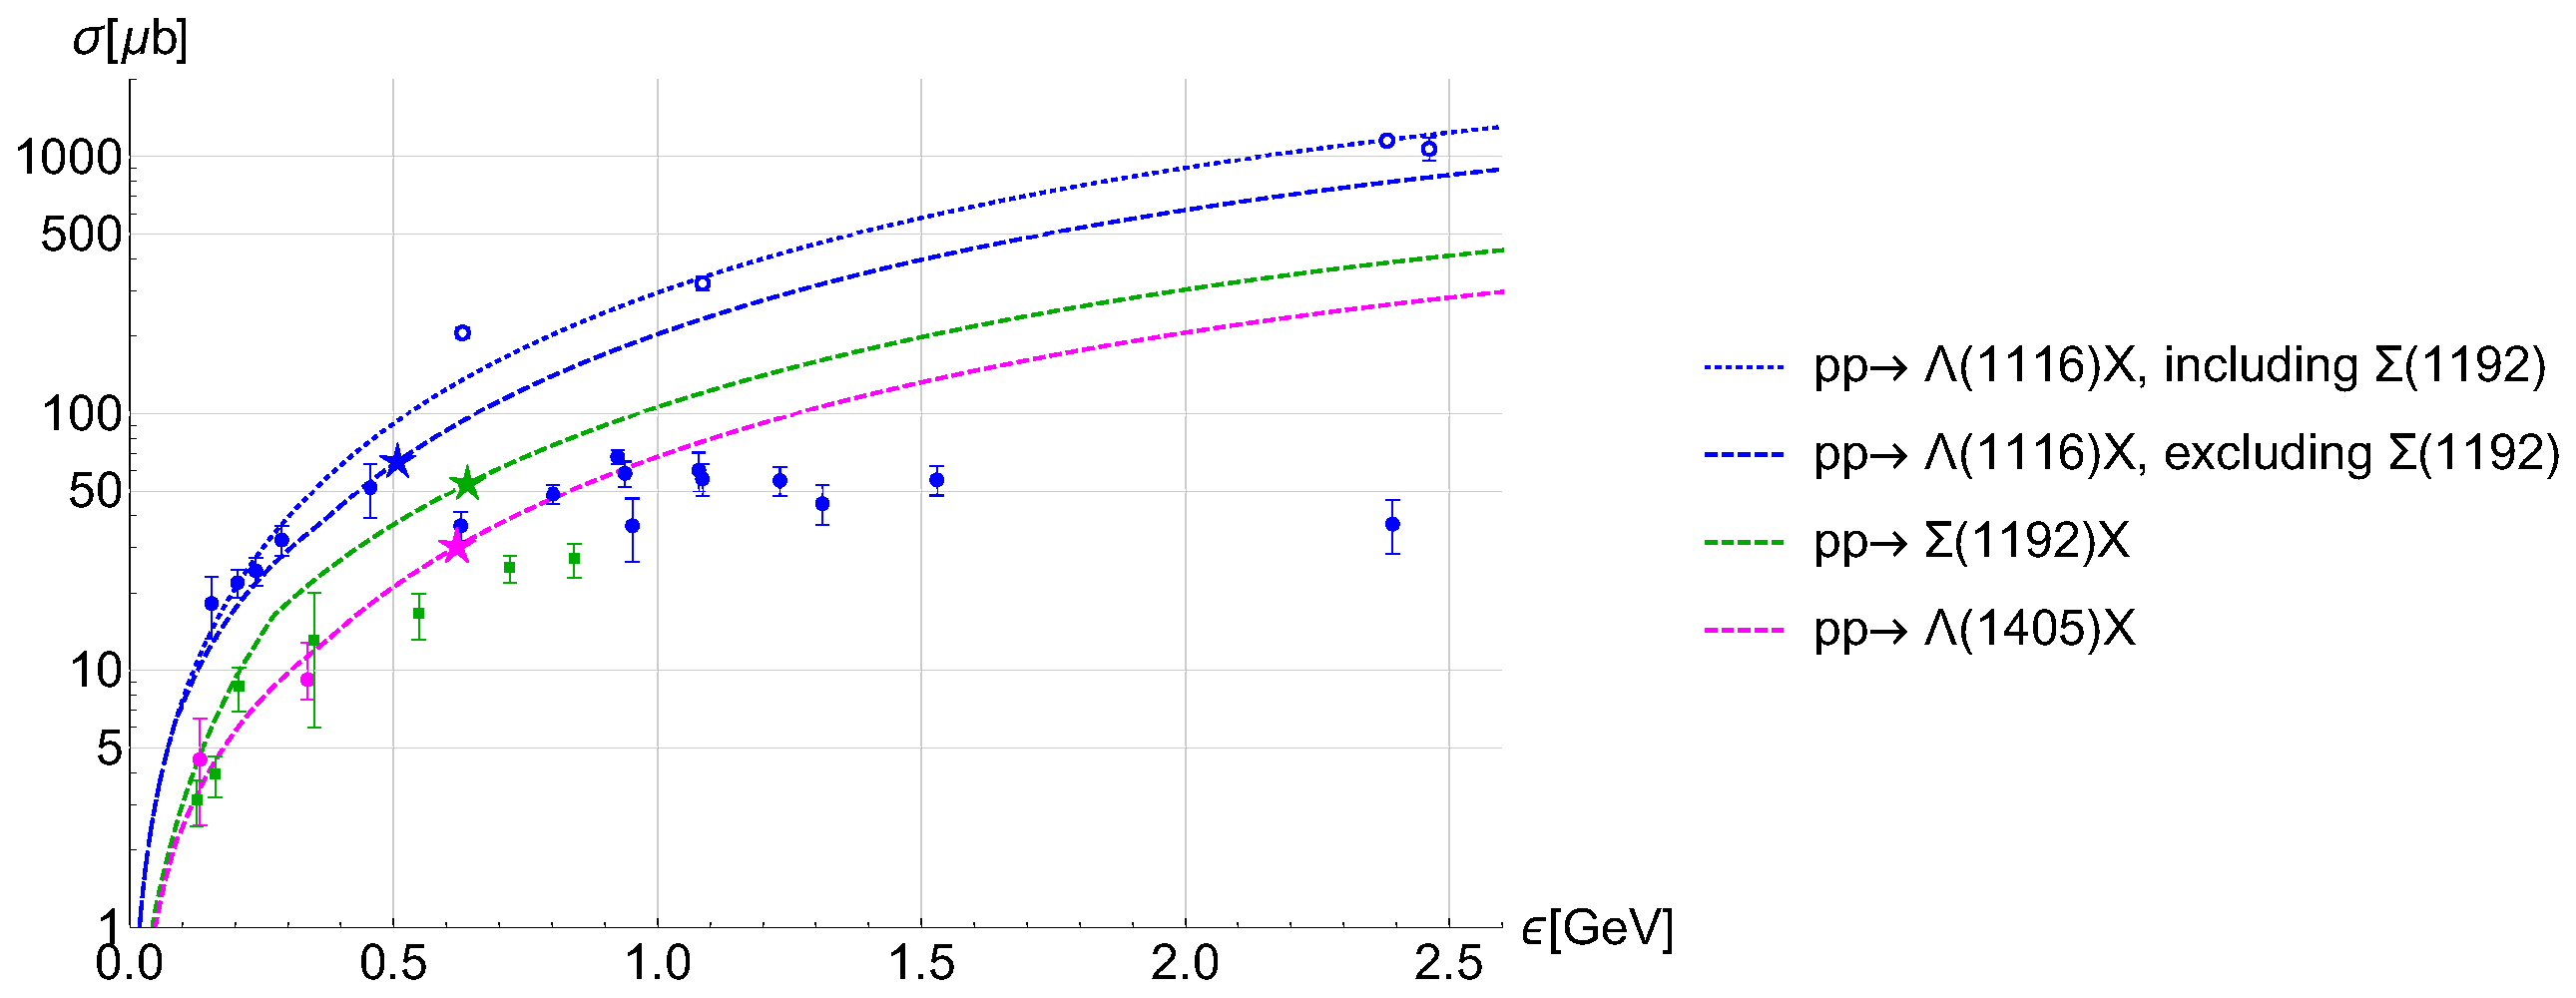
\includegraphics[width=0.9 \linewidth]{Chapter_simulation/all_CS}
  \caption{An estimated \css for Hyperons production. Blue dotted line shows an inclusive $\Lz$ production. It was decomposed into two components:i) $\Lz$ - blue dashed line and ii) $\Sz$ green dashed line. Magenta dashed line represents a parametrization of $\Lss$ \cs. All points refer to experimental data measured by different experiments \cite{L-B, COSY-TOF_L1405, COSY-TOF_SigmaLambda, hades_L1405, hades_inclL_35}. Color code is the same like for lines. Full points represent an exclusive \cs, empty points an inclusive one. }
  \label{fig:inclusive_cs}
\end{figure}

\subsection{$\Ls$, $\Lss$ and $\Ss$ production \css}
A knowledge about \css for $\L$ and $\S$ in function of $\Sqs$ or energy over the threshold $\e$ gives a possibility to estimate \cs for excited hyperon states. As a first approximation it was assumed that a production matrix element for ground and excited states is the same. It means that an only factor cases the difference in \cs is an avaliable energy over the treshold. It can be espressed by an equation
\begin{equation}
  \label{eq:cs_over_thr}
  \sigma_{\L^* X}(\L_{thr}^*+\eps)=\sigma_{\L X}(\L_{thr}+\eps),
\end{equation}
or in terms of $\Sqs$
\begin{equation}
  \sigma_{\L^* X}(\Sqs)=\sigma_{\L X}(\Sqs - \L^*_{thr}+\L_{thr}).
\end{equation}
Using the equation \ref{eq:cs_over_thr} I have calculated expected \css for the excided hyperons states $\Ls$ and $\Ss$. They are shown in \ref{fig:inclusive_cs} as blue and green star.  

A $\Lss$ exclusive \cs was mesured for two different energys by HADES \cite{hades_L1405} and COSY-tof \cite{COSY-TOF_L1405} experiment. In \cite{hades_L1405} outhors propozed a phenomentlogical parametrization of $\Lss$ exclusive \cs,
\begin{equation}
  \sigma^{excl}_{\Lss\p \Kp}(\eps)=\frac{1}{3}\sigma^{excl}_{\Lz \p \Kp}(\eps).
\end{equation}
I have followed the same relation for inclusive reactions multiplaying the inclusive $\Lz$ \cs by factor $1/3$. Result is shown in \ref{fig:inclusive_cs} by a magenta line. A magenta star shows point corresponding to $E_k=4.5 \mathrm{GeV}$ proton beam. Numerical values of the estimated \css are in tab. \ref{tab:sig_bg}.

\subsection{$\Xsi$}
Knowledge about a double-strange hyperon $\Xsi$ is extremly limited.
\section{Decay branching ratios}
Because Dalitz decays of hyperons were never measured a decay braching ratio have to be estimated considering avaliable data. A first approximation may be obtained using result for a non-strange sector. For a reaction $\Delta^+ \rightarrow \p \epem$ the HADES reported \cite{hades_Delta} $\mathrm{BR_{\Delta\rightarrow \p\epem}}=(4.19~\pm~0.62~\mathrm{~syst.}~\pm~0.34~\mathrm{~stat.})\times10^{-5}$. More precise estimation bases on, measured by CLAS collaboration \cite{Clas_Hyperons}, hyperons' radiative decays. A relation between radiative decays and Dalitz decays is given by the formula derived in F. Scozzi PhD thesis \cite{scozzi},
\begin{equation}
  \Gamma^{N^*\rightarrow~Ne^+e^-}=1.35 \cdot \alpha \Gamma^{N^*\rightarrow~N\gamma}.
\end{equation}
For $\Ls$ and $\Ss$ decay with for real photon decay are known. For $Lss$ the branchin ratio have to be astimted using other decay channels [ref]. Obtanied results (tab. \ref{tab:sig_bg}  are located in range of measured BR for $\Dp$ dalitz decay.


\section{Background channels selection}
To obtain a relaiablble simulation a coctail of background channels shoud be considered and tested. In case of hadronic physic, for low and medium enrgys, due to lack of approximation theorem, get a realistic background is a very challenging task. For a $\Sqs=$ 3.46 GeV a hadronic matter tends to form resonances. It means that almost all hadrons in final states originate from decays of high-mass resonances. Because knowledge about porperities of such a resonances is limited I made a simplified assumption that all pions are produced directly, without any intermediate state and with angular distribution defined jus by a reaction phase-space. List of all bacground channels considered during studies is presented in tab. \ref{tab:sig_bg}.

All channels considered as a $\Xsi$ background have to constist $\p \pim \pim$ in final state. A dominant one is a multi-pion production, however thanks to topological cuts (see chapter \ref{section:results}) this kind of the backgound is relatively easy to filter out. Second kind of the background considered in simulation is a $\Lz$ production associated with $\pim$. Reactions much more challenging because the $\Lz$ decay vertex is displaced from a target, the same like in signal reaction. \Css for channels numer 2-7 are taken from \cite{L-B}. When data in a proper energy range is missing, the value for the lowest avaliable enegry above $\Sqs=$ 3.46 GeV is taken. that conservative assumption gives me a save margin.

For all channels consisting of the hyperons' Dalitz decays a final state is the same: $\p \pim \epem$. That allows me to use the same background coctail for all three chanels. I divided possible bacground sources into three main grops. Firstly I considered a multi-pion production in a target area, channels: 14, 16 and 18. A di-lepton pair originates from a $\piz$ Dalitz decay and combination of $\p$ and $\pim$ creates false $\Lz$ signal. These channels differ from singal one mainly by a decay geometry. The $\Lz$ decays via week interaction with long lifetime $c\tau = 7.89$ cm \cite{PDG}, so its decay vertex is expected to be observed outside the target. A second group, channels 19, 21, 23, 24, 25, contains $\Lz$ production associated with a di-lepton source. In this case I have a real $\Lz$ and a $\epem$ pair coming from decay of different particles, mainly $\piz$. The \cs are taken from \cite{L-B}. The third source of background  are Dalitz decays of non-strange baryions associated with $\Lz$ production. The braching ratio was mesured only for $\Dp$ Dalitz \cite{hades_Delta}, for $\Dz$ Dalitz I have assumed the same value. A production \cs for the channels containing $\Delta$ has been calculated assumed that all pions comes from the reosnacnes decays. For example, channel 14 is the final state for reaction $\p\p \rightarrow p\Dp[\p\piz]\pip\pim$. Assuming that the $\Delta$ decay into pions conserv an izospin symmetry I used Clebsch-Gordan coefficients to calculate a ratio
\begin{equation}
  \frac{\Dp \rightarrow \p \piz}{\Dp \rightarrow \n\pip}=\frac{2}{1}.
\end{equation}
Hence, a total \cs for the reaction $\p\p \rightarrow p\Dp\pip\pim$ is $\frac{3}{2} \cdot \sigma_{pp \rightarrow \p\p \pip\pim\piz}$. The \css for other channels containing $\Delta$ dalitz decay were calculated in a similar way. Each $\Delta$ channel is listed below a reference multi-pion production channel. 

\begin{table}[!t]
  \centering
  \caption{List of signal (S) and background (B) channels for simulated reactions. Each channel containing $\Delta$ Dalitz decay is listed below reference channel, used for \cs estimation.}
  % \lineup
  \begin{tabular}{rlll}
    \hline
    no. &Channel & $\sigma$ [$\mu \barn$] & Type \\
    \hline
    \hline
    \multicolumn{4}{c}{$\Xsi$ production} \\
    \hline
    1&$\p\Kp\Kp\Xsi$                      & $\phantom{00}3.6/0.35$ & S \\
    \hline
    2&$\p\p\pip\pip \pim\pim$          & $\phantom{00}227$ & B  \\
    3&$\p\Lz\Kzs\pip$                  & $\phantom{00}30$ & B  \\
    4&$\p\Lz\Kp\pip\pim$               & $\phantom{00}21$ & B  \\
    5&$\neut\Lz\Kzs\pip\pip$           & $\phantom{00}10$ & B  \\
    6&$\p\Sz\Kzs\pip$                  & $\phantom{00}9$ & B  \\
    7&$\p\p\Kzs\Kzs$                   & $\phantom{00}1.6$ & B  \\

    %\multicolumn{4}{c}{$\dilambda$ production} \\
    %\hline
    %$\dilambda\Kp\Kp$                   & $\phantom{000}3.6/0.35$ & S \\
    %\hline
    %\multicolumn{4}{c}{background channels the same like for $\Xsi$ plus below} \\
    %$\p\p \Kp\Km$                    & $\phantom{00}20$ & B$^{\dagger}$ \\
    %\hline
    \hline
    \multicolumn{4}{c}{Dalitz decays of hyperons} \\
    \hline
    8&$\p\Kp\Ls[\Lz\epem]$          & $\phantom{0}69.6$, BR = \num{8.4e-5} & S \\
    9&$\p\Kp\Lss[\Lz\epem]$           & $\phantom{0}32.2$, BR = \num{5.3e-6} & S \\
    10&$\p\Kp\Ss[\Lz\epem]$           & $\phantom{0}56.24$, BR = \num{1.1e-4} & S \\
    \hline
    11&$\p\Kp\Ls[X]$                   & $\phantom{0}69.6$    & B  \\
    12&$\p\Kp\Lss[X]$                    & $\phantom{0}32.2$    & B  \\
    13&$\p\Kp\Ss[X]$                    & $\phantom{0}56.24$   & B  \\
    14&$\p\p \pip\pim\piz$              & $\phantom{0}1840$ & B \\
    15&$\p\pip\pim\Dp[\p\epem]$      & $\phantom{0}2760$, BR = \num{4.5e-5} & B  \\
    16&$\p\neut \pip\pip\pim\piz$          & $\phantom{0}300$      & B  \\
    17&$\p\pip\pip\pim\Dz[\neut \epem]$  & $\phantom{0}450$, BR = \num{4.5e-5} & B  \\
    18&$\p\p \pip\pim\piz\piz$          & $\phantom{0}300$      & B  \\
    19&$\p\Lz\Kp\piz$                   & $\phantom{0}43$      & B  \\
    20&$\Kp\Lz\Dp[\p\epem]$          & $\phantom{0}64$, BR = \num{4.5e-5} & B \\
    21&$\neut\Lz\Kp\pip\piz$               & $\phantom{0}20$      & B  \\
    22&$\pip\Kp\Lz\Dz[\neut\epem]$      & $\phantom{0}30$, BR = \num{4.5e-5} & B \\
    23&$\p\Lz\Kp\piz\piz$               & $\phantom{0}10$      & B  \\
    24&$\p\Sz\Kzs\pip$                  & $\phantom{0}9$      & B  \\
    25&$\p\Lz\Kp\piz\piz\piz$           & $\phantom{0}7$      & B  \\
    %\hline
    %\hline
    %\multicolumn{4}{c}{Real photon decays of hyperons} \\
    %\hline
    %$\p\Kp\Lss[\Lz\gamma]$        & $\phantom{00}69.6$, BR = \num{1.3e-2} & S \\
    %$\p\Kp\Ls[\Lz\gamma]$         & $\phantom{00}32.2$, BR = \num{5.0e-4} & S \\
    %$\p\Kp\Sstar[\Lz\gamma]$         & $\phantom{00}56.24$, BR = \num{1.1e-2} & S \\
    %\hline
    %$\p\p \pip\pim\piz$              & $\phantom{00}1840$    & B  \\
    %$\p\p \pip\pim\piz\piz$          & $\phantom{00}300$     & B  \\
    %$\p\Lz\Kp$                       & $\phantom{00}54.5$    & B$^{\ddagger}$ \\
    %$\p\Lz\Kp\piz$                   & $\phantom{00}43$      & B  \\
    %$\p\Lz\Kp\pip\pim$               & $\phantom{00}20$      & B  \\
    %$\p\Sz\Kp$                       & $\phantom{00}23.5$    & B$^{\ddagger}$ \\
    %$\p\Sz\Kp\piz$                   & $\phantom{00}20$      & B$^{\ddagger}$ \\
    %$\p\Sz\Kp\pip\pim$               & $\phantom{000}2$      & B$^{\ddagger}$ \\
    \hline
  \end{tabular}
  \label{tab:sig_bg}
\end{table}
\section{Simulations results}
The simulation has been performed usign folowing frameworks. The PLUTO event generator \cite{PLUTO1,PLUTO2} to simulate reactions in the target, the GEANT3 \cite{GEANT} software to simulate particles propagation through the detector and to simulate decay of unstable reaction's products like $\Lz$ or $\Kzs$. After all physics simulations, the detector answer and a full reconstruction chain was dane in the HYDRA framework. All together gives me a realistic simulation of an examineted physics, and the HADES behavour. The new HADES upgrades: new RICH, and the FwDet (see chapter \ref{chapter:HADES_upgrades}) were included.
\subsection{Particles identyfication}
\label{chapter:simulation_identyfication}
The particle identyfications algoritms used for simulation are, in principple, the same as for data collected during experiment. In first step all particle candidates are filtered to find events in wich track reconstracted in the MDC is fitted with the RICH rings. Additionally a Time-Of-Flight and Betha for leptonic track has to lay within a graphical cut. If both cryteria were fulfiled they are treated as lepton candidates. In next step for all non-leptnic candidates the mass is caltulated according to the formula
\begin{equation}
  m=\frac{pc}{\beta \gamma}.
\end{equation}
For protons and and pions the mass cuts are 650-1127 MeV and 40-240 MeV respectevly. 
\subsection{Hyperons Dalitz decays}

\subsection{Cascade decay}
\label{section:results}
\input{./Chapter_conclusions/conclusions.tex}
% \input{./Chapter2_symmetries/symmetries.tex} 
%\input{./Chapter4_test_kloe/test_kloe.tex} 
%\input{./Chapter5_test_jpet/test_jpet.tex} 
%\input{./Chapter3_detectors/detectors.tex}
%\input{./Chapter6_gps/gps.tex} 
%\input{./Chapter7_analysis_kloe/analysis_kloe.tex} 
%\input{./Chapter8_analysis_jpet/analysis_jpet.tex}
%\input{./Chapter9_conclusions/conclusions.tex}



%----------------------------------------------------------------------------------------
%	THESIS CONTENT - APPENDICES
%----------------------------------------------------------------------------------------
\addtocontents{toc}{\vspace{1em}} % Add a gap in the Contents, for aesthetics

%\appendix % Cue to tell LaTeX that the following 'chapters' are Appendices

% Include the appendices of the thesis as separate files from the Appendices folder
% Uncomment the lines as you write the Appendices
\begin{appendices}
%\chapter{The data-driven approach for a neural network training}
\label{appendix:data_driven}
The original paper by Metodiev, Nachman and Thaler \cite{Metodiev_2017} shows the idea of a data-driven analysis in details. Hire I want to introduce main concepts, necessery to understand how the proposed metode helps in the above analysis.





%%%Local Variables:
%%% TeX-master: "../main"
%%% End:
%\input{./Appendices/AppendixB}
%\input{./Appendices/AppendixC}
%\input{./Appendices/AppendixD}  
\end{appendices}

\addtocontents{toc}{\vspace{1em}} % Add a gap in the Contents, for aesthetics

%\backmatter

\cleardoublepage % Start a new page

%----------------------------------------------------------------------------------------%
%	ACKNOWLEDGEMENTS
%----------------------------------------------------------------------------------------
%\fancyhead[LO,RE]{\emph{Acknowledgements}} %
%\pagestyle{empty}
%\acknowledgements{%\addtocontents{toc}{\vspace{1em}} %Add a gap in the Contents, for aesthetics
%\input{./Acknowledgements}
%}

%----------------------------------------------------------------------------------------
%	BIBLIOGRAPHY
%---------------------------------------------------------------------------------------- 
\cleardoublepage
\pagestyle{fancy}
%\fancyhead[LO,RE]{\emph{\leftmark}} % Set the left side page header to chapter title
\addtotoc{\bf Bibli
ography}
\label{Bibliography}
%\lhead{\emph{Bibliography}} % Change the page header to say "Bibliography"

\setstretch{1.1} % Line spacing of 1.3
 \bibliographystyle{utphys}
%\bibliographystyle{mybibstyle}

%\bibliography{bibtex/theory,bibtex/misc,bibtex/kloe,bibtex/jpet} % The references (bibliography) information are stored in the file named "Bibliography.bib"
\bibliography{bibtex/hades}
% \begin{thebibliography}{99}
% \input{./Other/References.tex}
% \end{thebibliography}

\end{document}  
